%% LyX 2.0.6 created this file.  For more info, see http://www.lyx.org/.
%% Do not edit unless you really know what you are doing.
\documentclass[10pt,english]{beamer}
\usepackage[T1]{fontenc}
\usepackage[utf8]{luainputenc}
\usepackage{babel}
\usepackage{amsmath}
\usepackage{amssymb}
\usepackage{graphicx}
\usepackage{esint}
\ifx\hypersetup\undefined
  \AtBeginDocument{%
    \hypersetup{unicode=true,pdfusetitle,
 bookmarks=true,bookmarksnumbered=true,bookmarksopen=true,bookmarksopenlevel=1,
 breaklinks=false,pdfborder={0 0 0},backref=false,colorlinks=true,
 linkcolor=black, citecolor=black}
  }
\else
  \hypersetup{unicode=true,pdfusetitle,
 bookmarks=true,bookmarksnumbered=true,bookmarksopen=true,bookmarksopenlevel=1,
 breaklinks=false,pdfborder={0 0 0},backref=false,colorlinks=true,
 linkcolor=black, citecolor=black}
\fi

\makeatletter
\@addtoreset{subfigure}{framenumber}
%%%%%%%%%%%%%%%%%%%%%%%%%%%%%% LyX specific LaTeX commands.
%% Because html converters don't know tabularnewline
\providecommand{\tabularnewline}{\\}

%%%%%%%%%%%%%%%%%%%%%%%%%%%%%% Textclass specific LaTeX commands.
 % this default might be overridden by plain title style
 \newcommand\makebeamertitle{\frame{\maketitle}}%
 \AtBeginDocument{
   \let\origtableofcontents=\tableofcontents
   \def\tableofcontents{\@ifnextchar[{\origtableofcontents}{\gobbletableofcontents}}
   \def\gobbletableofcontents#1{\origtableofcontents}
 }
 \long\def\lyxframe#1{\@lyxframe#1\@lyxframestop}%
 \def\@lyxframe{\@ifnextchar<{\@@lyxframe}{\@@lyxframe<*>}}%
 \def\@@lyxframe<#1>{\@ifnextchar[{\@@@lyxframe<#1>}{\@@@lyxframe<#1>[]}}
 \def\@@@lyxframe<#1>[{\@ifnextchar<{\@@@@@lyxframe<#1>[}{\@@@@lyxframe<#1>[<*>][}}
 \def\@@@@@lyxframe<#1>[#2]{\@ifnextchar[{\@@@@lyxframe<#1>[#2]}{\@@@@lyxframe<#1>[#2][]}}
 \long\def\@@@@lyxframe<#1>[#2][#3]#4\@lyxframestop#5\lyxframeend{%
   \frame<#1>[#2][#3]{\frametitle{#4}#5}}
 \def\lyxframeend{} % In case there is a superfluous frame end
 \newenvironment{topcolumns}{\begin{columns}[t]}{\end{columns}}

%%%%%%%%%%%%%%%%%%%%%%%%%%%%%% User specified LaTeX commands.
\usepackage{cite}
\usepackage{notoccite}




\usepackage{babel}
%\usepackage{xunicode}

\@ifundefined{showcaptionsetup}{}{%
 \PassOptionsToPackage{caption=false}{subfig}}
\usepackage{subfig}
\makeatother

\begin{document}

\title{\emph{Ab initio} Calculations of Intramolecular Exciton Transfer with Reduced Modes in Donor-Bridge-Acceptor Species}


\author{Xunmo Yang}

\makebeamertitle

\lyxframeend{}\lyxframe{Outline}
\begin{itemize}
\item Introduction
\item Benchmark of TCLME with Edmiston-Ruedenberg diabatization
\item Primary Mode
\item Application in IR-controlled electron transfer
\item Conclusions
\end{itemize}

\lyxframeend{}



\lyxframeend{}\lyxframe{Electron Transfer}

\begin{figure}[t]
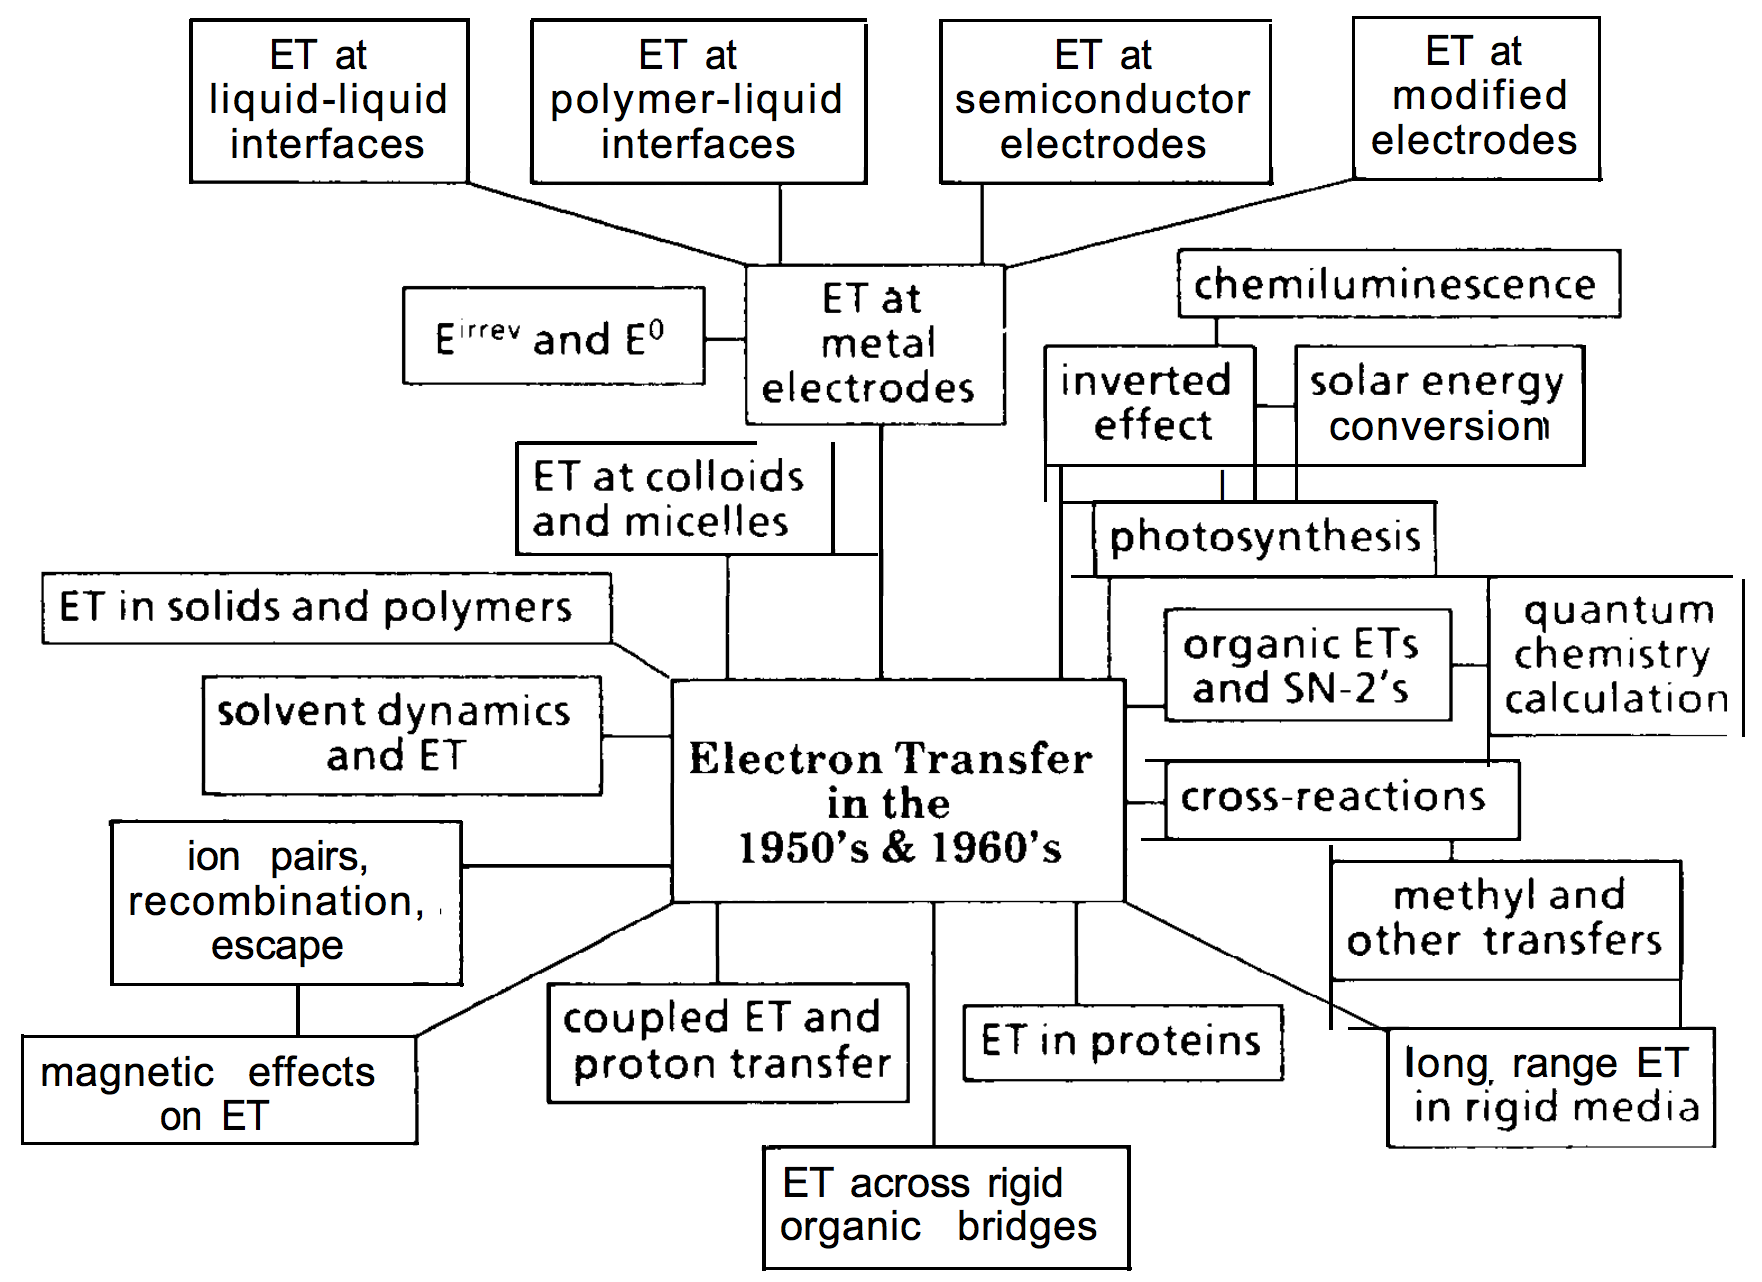
\includegraphics[width=0.9\columnwidth]{ET_application.png}
\end{figure}

\small{Rudolph A. Marcus - Nobel Lecture: Electron Transfer Reactions in Chemistry: Theory and Experiment".}
\lyxframeend{}


\lyxframeend{}\lyxframe{Marcus Theory}
\begin{topcolumns}%{}


\column{7cm}

Energy and electronic transport is fundamental in chemistry. The seminal model for calculating transfer rates was developed by Marcus.
\[
H_{dia}=\hat{T_{n}}+\left(\begin{array}{cc}
\epsilon_{a}(\mathbf{R}) & V_{ab}\\
V_{ab} & \epsilon_{b}(\mathbf{R})
\end{array}\right)
\]



\[
k_{Marcus}=\frac{2\pi}{\hbar}|V_{ab}|^{2}\frac{1}{\sqrt{4\text{\ensuremath{\pi}}k_{B}T\lambda}}e^{-(\lambda+\Delta E)^{2}/4\text{\ensuremath{\lambda}}k_{B}T}
\]

\begin{itemize}
\item Condon approximation:$V_{ab}(\mathbf{R})=V_{ab}$
\item All vibrations are included in a collective coordinate
\item $k_{B}T \gg \hbar \omega$
\end{itemize}

\column{4cm }


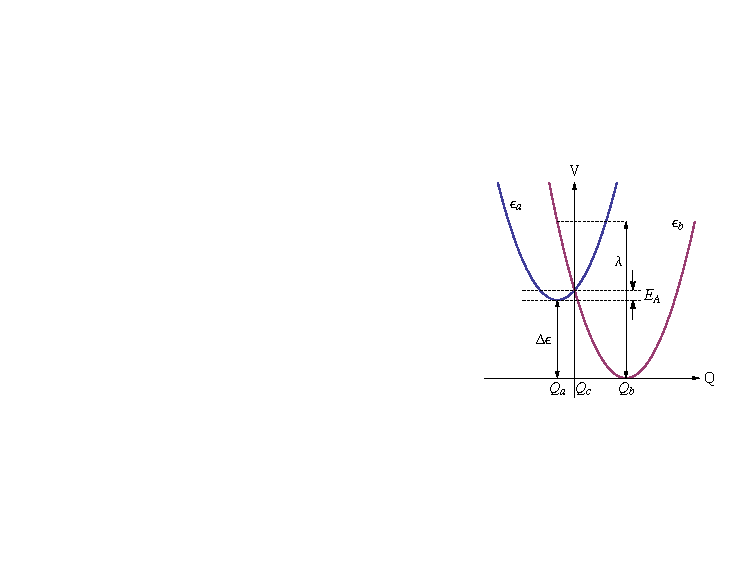
\includegraphics[height=4cm]{Chapters/chap2/Figure1}

\end{topcolumns}%{}

\lyxframeend{}



\lyxframeend{}\lyxframe{Adiabatic vs. Diabatic Representation}


\begin{figure}


\begin{centering}
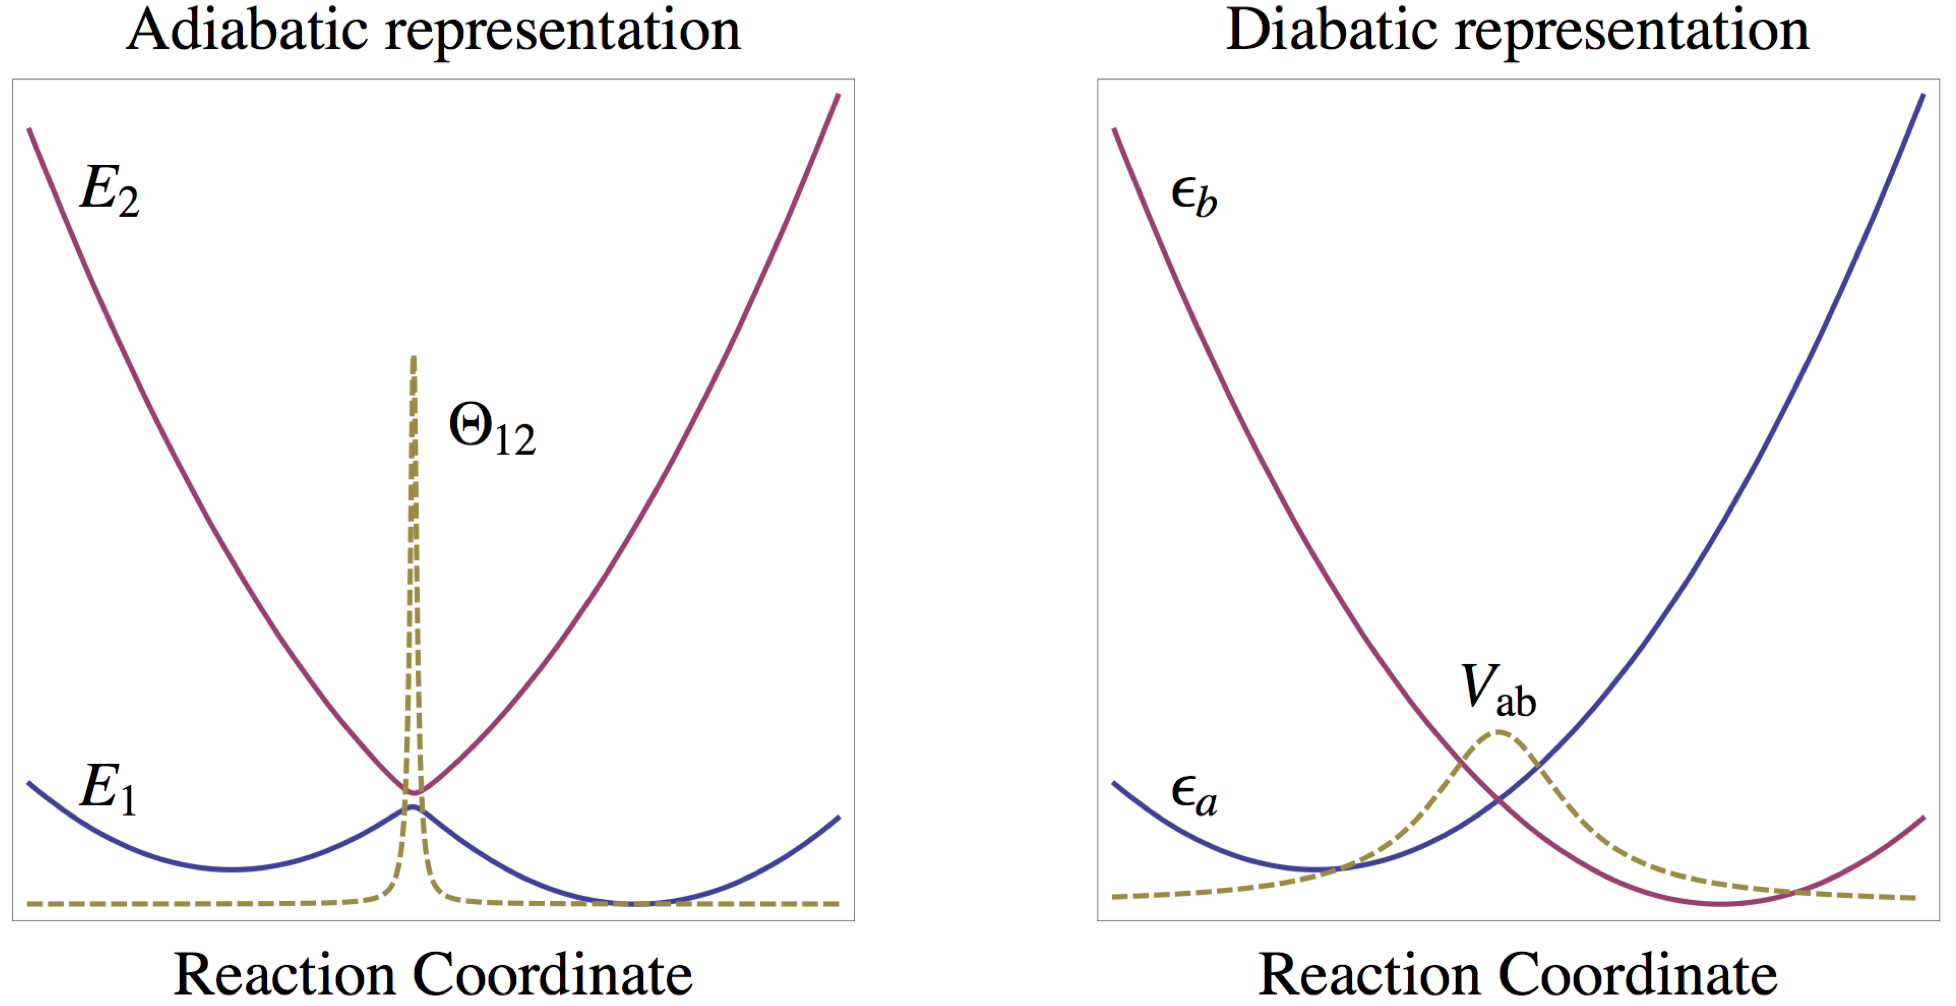
\includegraphics[width=0.7\textwidth]{Chapters/chap2/adia_vs_diabatic.png}
\par\end{centering}

\end{figure}

Adiabatic representation

Pros:
\begin{itemize}
\item Eigenstate of electronic Hamiltonian, directly available from quantum chemistry software
\end{itemize}
Cons:
\begin{itemize}
\item Potential energy surfaces aren't parabolic (avoided crossing)
\item Sharp derivative coupling near avoided crossing (hard to compute)
\end{itemize}


\lyxframeend{}



\lyxframeend{}\lyxframe{Diabatization: Boys \& Edmiston-Ruedenberg Localization}

\[
H_{adia}=\begin{pmatrix}E_{1}(\mathbf{R})+\mathrm{T_{n}}(\mathbf{R})_{11} & \mathrm{T_{n}}(\mathbf{R})_{12}\\
\mathrm{T_{n}}(\mathbf{R})_{21} & E_{2}(\mathbf{R})+\mathrm{T_{n}}(\mathbf{R})_{22}
\end{pmatrix}
\]


Construct diabatic states to eliminate dynamical coupling,
\begin{itemize}
\item Exact way $\left\langle \phi_{i}(\mathbf{r};\mathbf{R})|\nabla_{\mathbb{\mathbf{R}}}|\phi_{j}(\mathbf{r};\mathbf{R})\right\rangle =0$
(expensive \& rarely exist)
\item Intuitive way. Transform $H_{adia}$
\end{itemize}
\[
H_{dia}=U^{T}H_{adia}U=\left(\begin{array}{cc}
\epsilon_{a}(\mathbf{R})\mathrm{+T'_{n}}(\mathbf{R})_{11} & V_{ab}(\mathbf{R})\\
V_{ab}(\mathbf{R}) & \epsilon_{b}(\mathbf{R})\mathrm{+T'_{n}}(\mathbf{R})_{22}
\end{array}\right)
\]


to maximize/minimize certain physical property

\[
f_{Boys}=\sum_{kl}^{N_{states}}\left(\left\langle \phi_{k}|\vec{r}|\phi_{k}\right\rangle -\left\langle \phi_{l}|\vec{r}|\phi_{l}\right\rangle \right)^{2}
\]


\textrm{
\[
f_{ER}=\sum_{k}^{N_{states}}\iint \! \mathrm{d}r_{1}\mathrm{d}r_{2}\frac{\left\langle \phi_{k}|\hat{\rho}\left(r_{1}\right)|\phi_{k}\right\rangle \left\langle \phi_{k}|\hat{\rho}\left(r_{2}\right)|\phi_{k}\right\rangle }{\left\Vert r_{1}-r_{2}\right\Vert }
\]
}


\lyxframeend{}




\lyxframeend{}\lyxframe{Diabatization: Generalized Mulliken Hush (GMH)}

\[
\begin{pmatrix} |\phi_{a}\rangle\\|\phi_{b}\rangle\end{pmatrix}
= U^{T}\begin{pmatrix} |\psi_{1}\rangle\\|\psi_{2}\rangle\end{pmatrix}
= \left(\begin{array}{cc}
\cos\theta & \sin\theta\\
-\sin\theta & \cos\theta
\end{array}\right)
\begin{pmatrix} |\psi_{1}\rangle\\|\psi_{2}\rangle\end{pmatrix}
\]


Assuming only the direction along $\vec{\mu}_{11} - \vec{\mu}_{22}$ matters, we project all dipole moments onto $\vec{v} = (\vec{\mu}_{11} - \vec{\mu}_{22})/|\vec{\mu}_{11} - \vec{\mu}_{22}|$.
% \[\mu_{ab} = \langle\phi_{a}| \vec{\mu} | \phi_{b}\rangle
% = \cos2\theta \vec{\mu}_{12} - \frac{1}{2}\sin2\theta(\vec{\mu}_{11} - \vec{\mu}_{22})
% \]
\[\mu_{ab}^{v} = \langle\phi_{a}| \vec{\mu} | \phi_{b}\rangle \cdot \vec{v}
= \cos2\theta \vec{\mu}_{12}^{v} - \frac{1}{2}\sin2\theta|\vec{\mu}_{11} - \vec{\mu}_{22}|
\]
Good diabatic states should have $\mu_{ab}^{v} = 0$, this determines $\theta$ and gives
% \[\tan2\theta=\frac{2\mu_{12}^v}{|\vec{\mu}_{11} - \vec{\mu}_{22}|}
% \]
\[|H_{AB}|=|\cos2\theta {H}_{12} - \frac{1}{2}\sin2\theta({H}_{11} - {H}_{22})|
= \frac{|\mu_{12}^{v}||H_{11}-H_{22}|}{\sqrt{|\vec{\mu}_{11} - \vec{\mu}_{22}|^2 + 4|\mu_{12}^{v}|^2}}
\]
For linear systems, we further assume $|\mu_{12}^{v}| = |\mu_{12}|$.

\lyxframeend{}



\lyxframeend{}\lyxframe{Time-convolutionless Master Equation (TCLME)}

Bittner and Pereversev developed TCLME for Hamiltonian
\[
H=\left(\begin{array}{cc}
E_{a}\\
 & E_{b}
\end{array}\right)+\sum_{ijq}g_{ijq}|\phi_{i}\rangle\langle\phi_{j}|q+\sum_{q}\hbar\omega_{q}(n+1/2)
\]


To get this desired form, we assume diabatic potentials are the parabolas
same as adiabatic potentials, then at $Q_{b}$,

\[
H_{dia}=\left(\begin{array}{cc}
\epsilon_{a} & V_{ab}\\
V_{ab} & \epsilon_{b}
\end{array}\right)+\left(\begin{array}{cc}
\\
 & \sum_{i}g_{22i}q_{i}
\end{array}\right)+h.o.
\]


% Use $U=\left(\begin{array}{cc}
% \cos\theta & -\sin\theta\\
% \sin\theta & \cos\theta
% \end{array}\right)$ to
Diagonalize the electronic part
\[
H=U^{T}H_{dia}U=\left(\begin{array}{cc}
E_{a}\\
 & E_{b}
\end{array}\right)+\left(\begin{array}{cc}
\sin^{2}\theta & \frac{1}{2}\sin2\theta\\
\frac{1}{2}\sin2\theta & \cos^{2}\theta
\end{array}\right)\sum_{i=1}^{NMode}g_{22i}q_{i}+h.o.
\]



\lyxframeend{}



\lyxframeend{}\lyxframe{Validity of Assumptions}

\begin{figure}
\subfloat{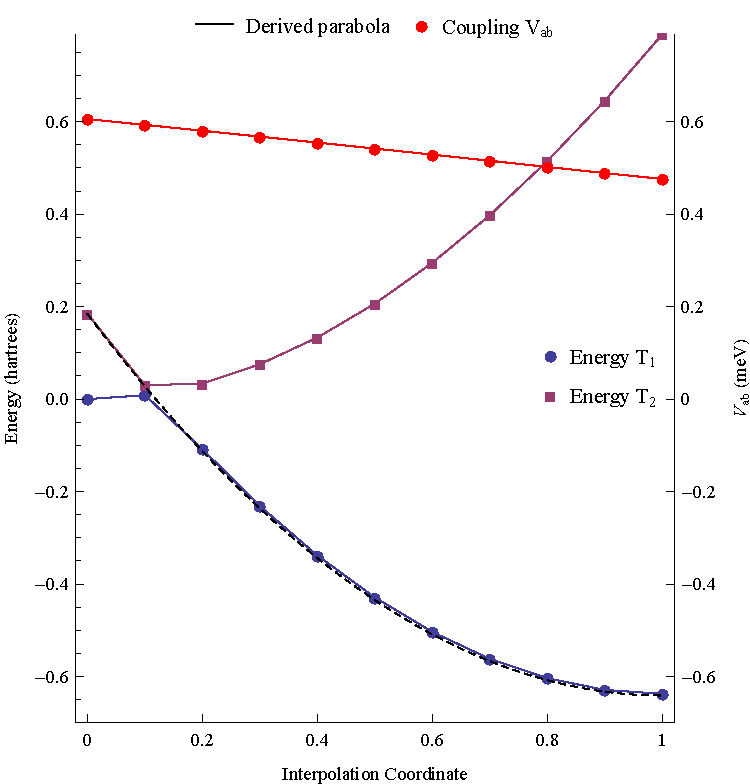
\includegraphics[width=0.4\columnwidth]{Chapters/chap2/Figure2a}}
\subfloat{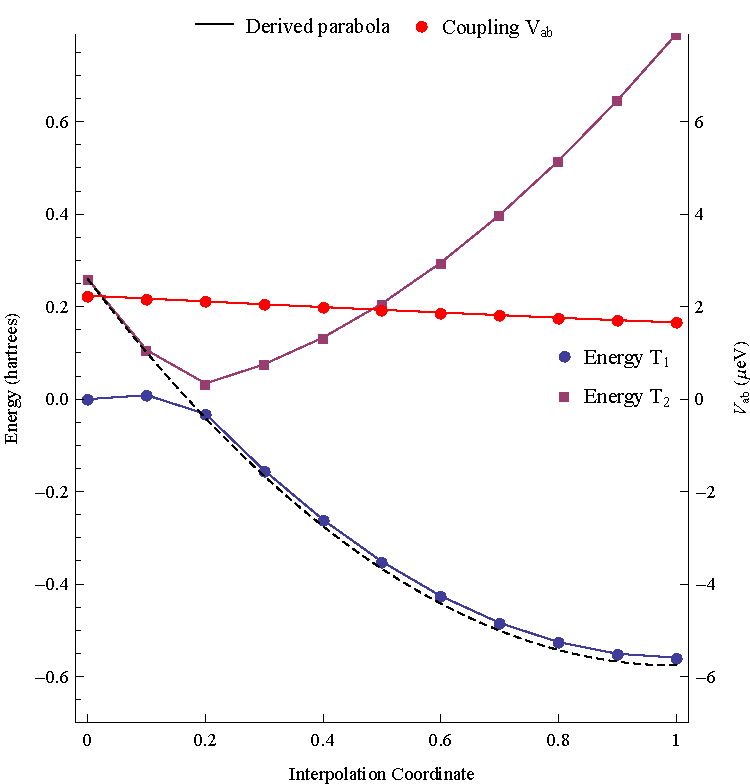
\includegraphics[width=0.4\columnwidth]{Chapters/chap2/Figure2b}}
\caption{Adiabatic energy curves and off-diagonal couplings computed along an interpolation coordinate between the
$D^{*}-B-A$ and $D-B-A^{*}$ equilibrium geometries for (a) c-1,4ee and (b) d-2,6ae.}
\end{figure}
\begin{itemize}
\item Condon approximation: diabatic couplings are small \& steady
\item Parabolic assumption holds well
\end{itemize}

\lyxframeend{}

\lyxframeend{}\lyxframe{Benchmark with Closs' Experiments}

\begin{table}
\caption{Transfer rates obtained from experiments, TCLME and Marcus theory.\label{tab:Transfer rates}}


% \noindent \begin{raggedright}
% \begin{tabular}{|c|c|c|c|c|c|}
% \hline
% Symbol & Structure & $k_{e}\left(1/s\right)$ & $k_{T}\left(1/s\right)$ & $k_{M}\left(1/s\right)$ & $V_{ab}\left(meV\right)$\tabularnewline
% \hline
% \hline
% c-1,3ee & \includegraphics[height=0.35cm]{\string"Chapters/chap2/Table1-c13ee\string".pdf} & $7.7\times10^{9}$ & $2.8\times10^{10}$ & $2.1\times10^{10}$ & $1.6$\tabularnewline
% \hline
% c-1,4ee & \includegraphics[height=0.35cm]{\string"Chapters/chap2/Table1-c14ee\string".pdf} & $1.3\times10^{9}$ & $4.0\times10^{9}$ & $3.9\times10^{9}$ & $0.61$\tabularnewline
% \hline
% c-1,3ea & \includegraphics[height=0.7cm]{\string"Chapters/chap2/Table1-c13ea\string".pdf} & $3.3\times10^{9}$ & $5.0\times10^{9}$ & $3.9\times10^{9}$ & $0.7$\tabularnewline
% \hline
% d-2,6ae & \includegraphics[height=0.7cm]{\string"Chapters/chap2/Table1-d26ae\string".pdf} & $1.3\times10^{5}$ & $5.5\times10^{4}$ & $1.0\times10^{4}$ & $0.0023$\tabularnewline
% \hline
% d-2,6ea & \includegraphics[height=0.7cm]{\string"Chapters/chap2/Table1-d26ea\string".pdf} & $7\times10^{5}$ & $0.7$ & $3.9\mathbf{\times}10^{4}$       & $8.2\times10^{-6}$\tabularnewline
% \hline
% d-2,7ea & \includegraphics[height=0.7cm]{\string"Chapters/chap2/Table1-d27ea\string".pdf} & $1.5\times10^{7}$ & $3.0\times10^{7}$ & $1.8\times10^{7}$ & $0.7$\tabularnewline
% \hline
% \end{tabular}
% \par\end{raggedright}

% \includegraphics[height=1.5cm]{\string"fig/chemical structure/bridge\string".pdf}
% \end{table}



\noindent \begin{raggedright}
\begin{tabular}{|c|c|c|c|c|c|}
\hline
Symbol & Structure & $k_{expr}\left(1/s\right)$ & $k_{Marcus}\left(1/s\right)$ & $k_{TCLME}\left(1/s\right)$ \tabularnewline
\hline
 c-1,3ea  &  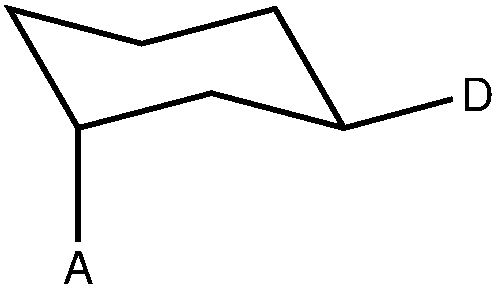
\includegraphics[height=0.7cm]{Chapters/chap2/Table1-c13ea.pdf}  &                     3.3E9  &                     3.9E9  &          2.2E9   \\
\hline
 c-1,3ee  &  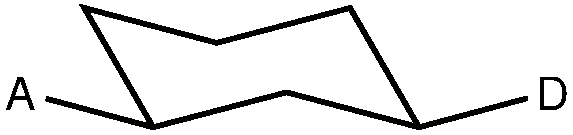
\includegraphics[height=0.35cm]{Chapters/chap2/Table1-c13ee.pdf}  &                     7.7E9  &                    2.1E10  &         2.8E10   \\
\hline
 c-1,4ea  &  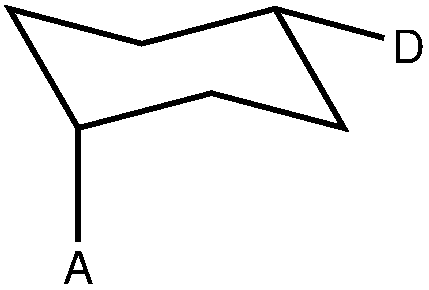
\includegraphics[height=0.7cm]{Chapters/chap2/Table1-c14ea.pdf}  &                     4.0E7  &                     1.3E7  &          1.8E7  \\
\hline
 c-1,4ee  &  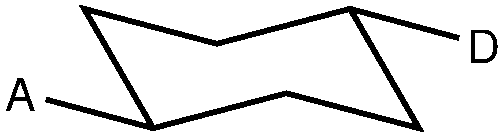
\includegraphics[height=0.35cm]{Chapters/chap2/Table1-c14ee.pdf}  &                     1.3E9  &                     3.9E9  &          3.6E9   \\
\hline
 d-2,6ae  &  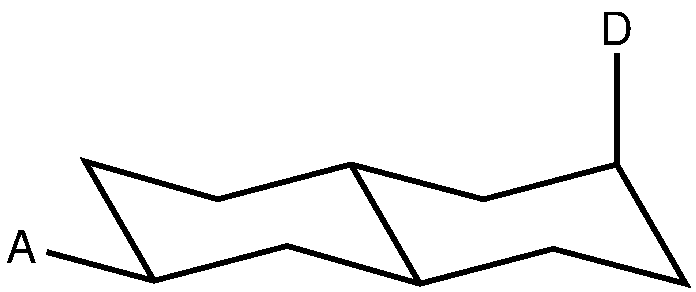
\includegraphics[height=0.7cm]{Chapters/chap2/Table1-d26ae.pdf}  &                     1.3E5  &                     1.0E4  &          4.7E4 \\
% \hline
% d-2,6ea  &  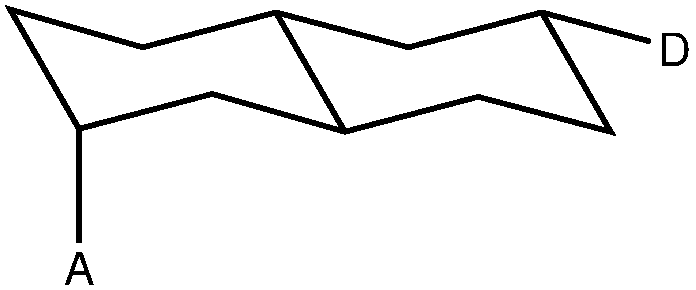
\includegraphics[height=0.7cm]{Chapters/chap2/Table1-d26ea.pdf}  &                     7.0E5  &                     3.9E4  &          5.8E4   \\
% \hline
%  d-2,6ee  &  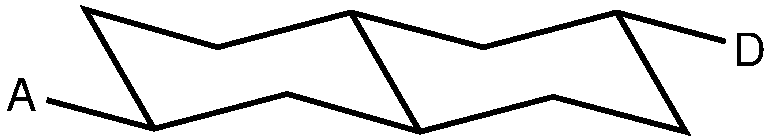
\includegraphics[height=0.35cm]{Chapters/chap2/Table1-d26ee.pdf}  &                     3.1E6  &                     5.0E6  &          4.8E6  \\
% \hline
%  d-2,7ae  &  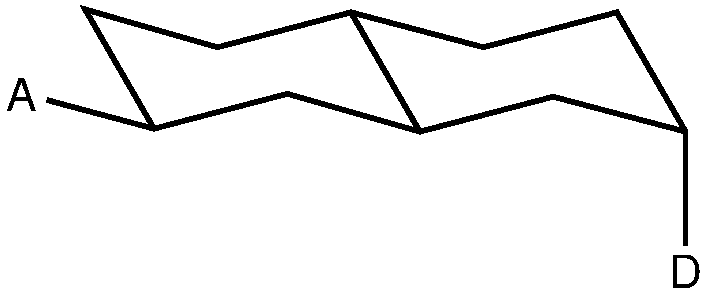
\includegraphics[height=0.35cm]{Chapters/chap2/Table1-d27ae.pdf}  &                     1.1E7  &                     2.8E7  &          3.0E7   \\
% \hline
%  d-2,7ea  &  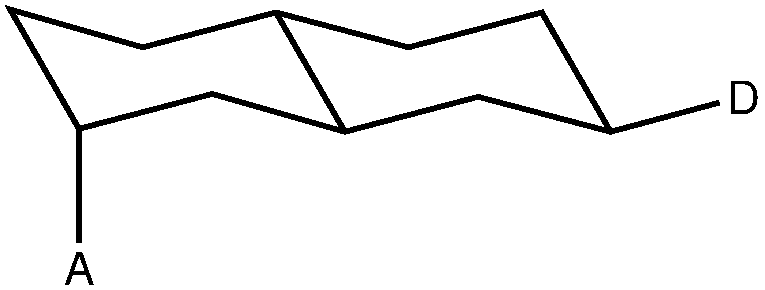
\includegraphics[height=0.7cm]{Chapters/chap2/Table1-d27ea.pdf}  &                     1.5E7  &                     1.8E7  &          4.3E7  \\
% \hline
%  d-2,7ee  &  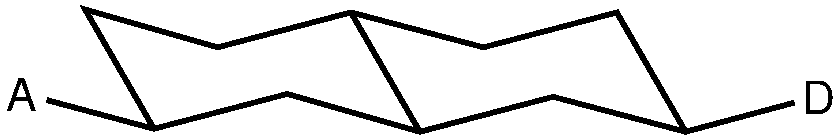
\includegraphics[height=0.35cm]{Chapters/chap2/Table1-d27ee.pdf}  &                     9.1E7  &                     3.5E8  &          3.4E8  \\
% \hline
%  M        &  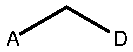
\includegraphics[height=0.35cm]{Chapters/chap2/Table1-M.pdf}      &                    5.0E10  &                      n.r.  &          1.2E9  \\
\hline
\end{tabular}
\par\end{raggedright}
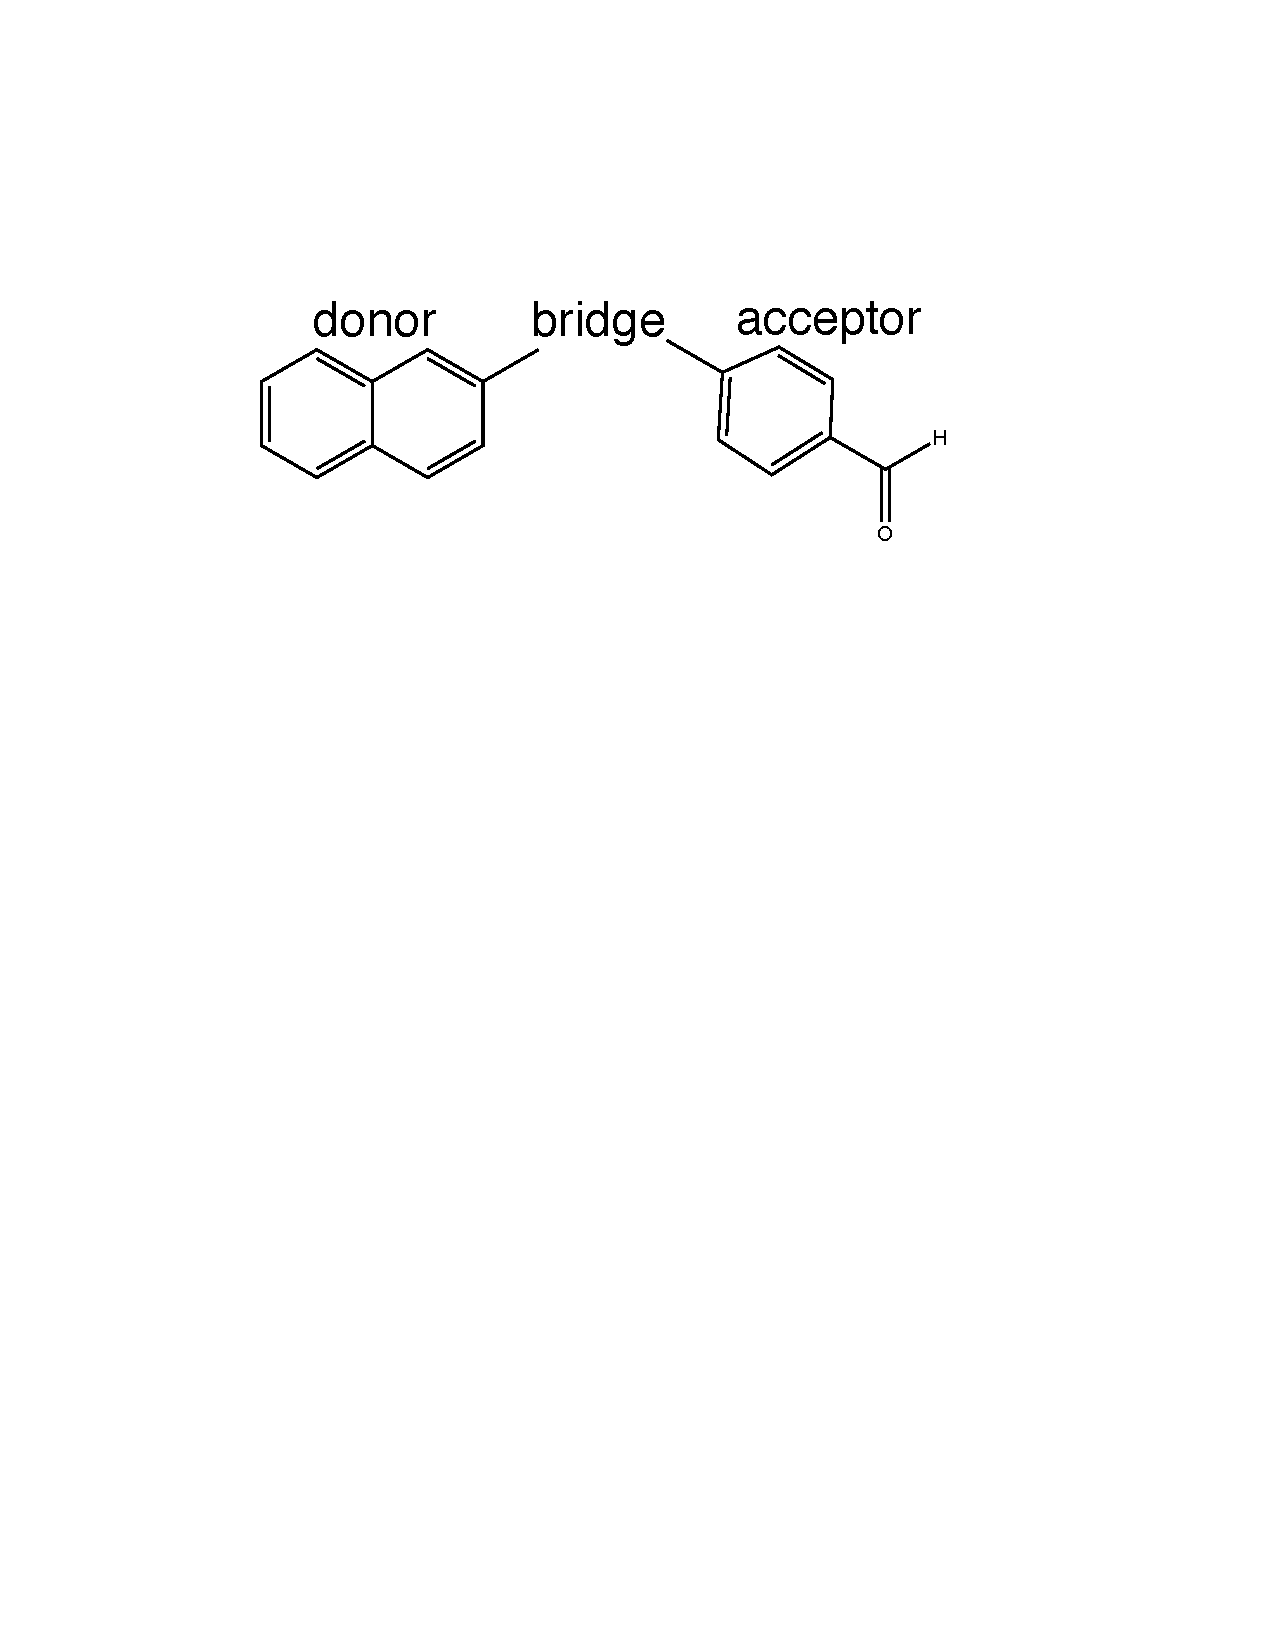
\includegraphics[height=1.5cm]{Chapters/chap2/Scheme1}
\end{table}

\lyxframeend{}



\lyxframeend{}\lyxframe{Benchmark with Closs' Experiments (Cont'd)}

\begin{table}
% \caption{Transfer rates obtained from experiments, TCLME and Marcus theory.\label{tab:Transfer rates}}
\noindent \begin{raggedright}
\begin{tabular}{|c|c|c|c|c|c|}
\hline
Symbol & Structure & $k_{expr}\left(1/s\right)$ & $k_{Marcus}\left(1/s\right)$ & $k_{TCLME}\left(1/s\right)$ \tabularnewline
\hline
%  c-1,3ea  &  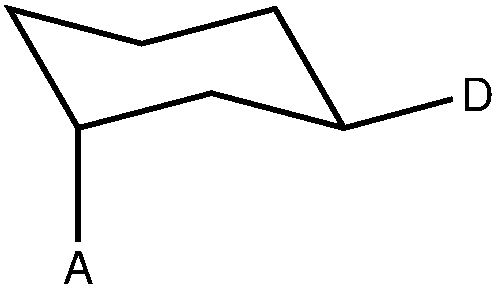
\includegraphics[height=0.7cm]{Chapters/chap2/Table1-c13ea.pdf}  &                     3.3E9  &                     3.9E9  &          2.2E9   \\
% \hline
%  c-1,3ee  &  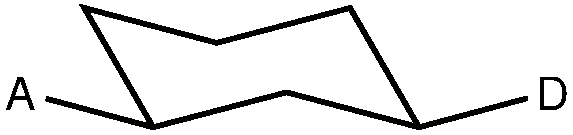
\includegraphics[height=0.35cm]{Chapters/chap2/Table1-c13ee.pdf}  &                     7.7E9  &                    2.1E10  &         2.8E10   \\
% \hline
%  c-1,4ea  &  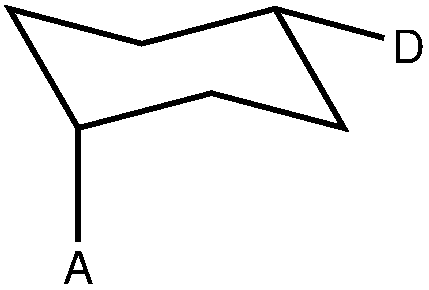
\includegraphics[height=0.7cm]{Chapters/chap2/Table1-c14ea.pdf}  &                     4.0E7  &                     1.3E7  &          1.8E7  \\
% \hline
%  c-1,4ee  &  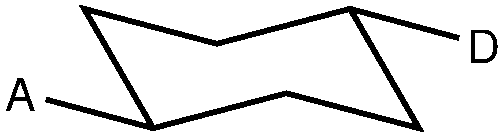
\includegraphics[height=0.35cm]{Chapters/chap2/Table1-c14ee.pdf}  &                     1.3E9  &                     3.9E9  &          3.6E9   \\
% \hline
%  d-2,6ae  &  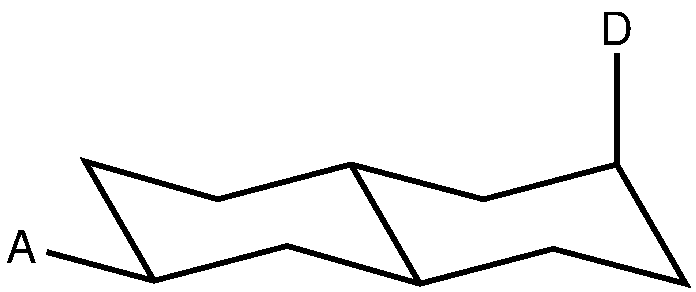
\includegraphics[height=0.35cm]{Chapters/chap2/Table1-d26ae.pdf}  &                     1.3E5  &                     1.0E4  &          4.7E4 \\
\hline
d-2,6ea  &  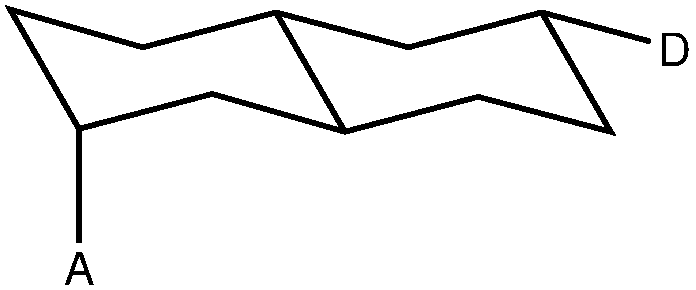
\includegraphics[height=0.7cm]{Chapters/chap2/Table1-d26ea.pdf}  &                     7.0E5  &                     3.9E4  &          5.8E4   \\
\hline
 d-2,6ee  &  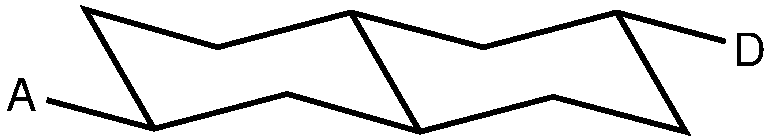
\includegraphics[height=0.35cm]{Chapters/chap2/Table1-d26ee.pdf}  &                     3.1E6  &                     5.0E6  &          4.8E6  \\
\hline
 d-2,7ae  &  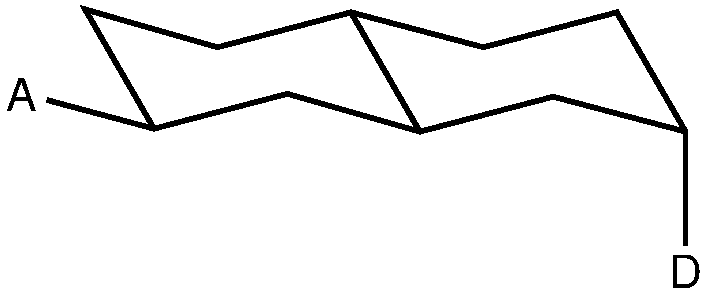
\includegraphics[height=0.7cm]{Chapters/chap2/Table1-d27ae.pdf}  &                     1.1E7  &                     2.8E7  &          3.0E7   \\
\hline
 d-2,7ea  &  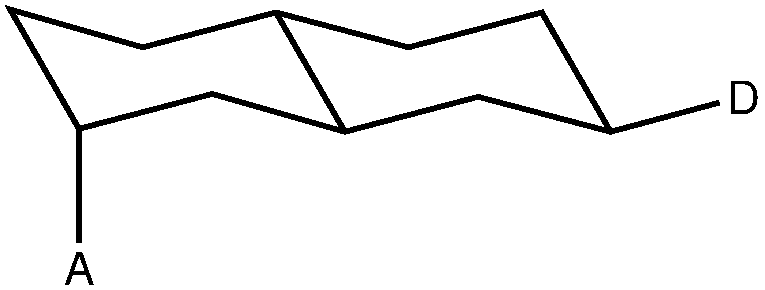
\includegraphics[height=0.7cm]{Chapters/chap2/Table1-d27ea.pdf}  &                     1.5E7  &                     1.8E7  &          4.3E7  \\
\hline
 d-2,7ee  &  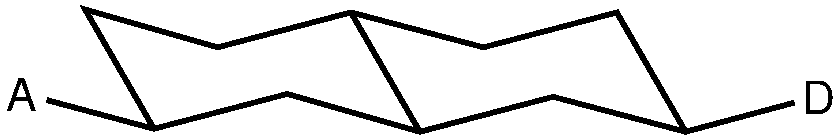
\includegraphics[height=0.35cm]{Chapters/chap2/Table1-d27ee.pdf}  &                     9.1E7  &                     3.5E8  &          3.4E8  \\
\hline
 M        &  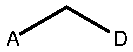
\includegraphics[height=0.35cm]{Chapters/chap2/Table1-M.pdf}      &                    5.0E10  &                      n.r.  &          1.2E9  \\
\hline
\end{tabular}
\par\end{raggedright}
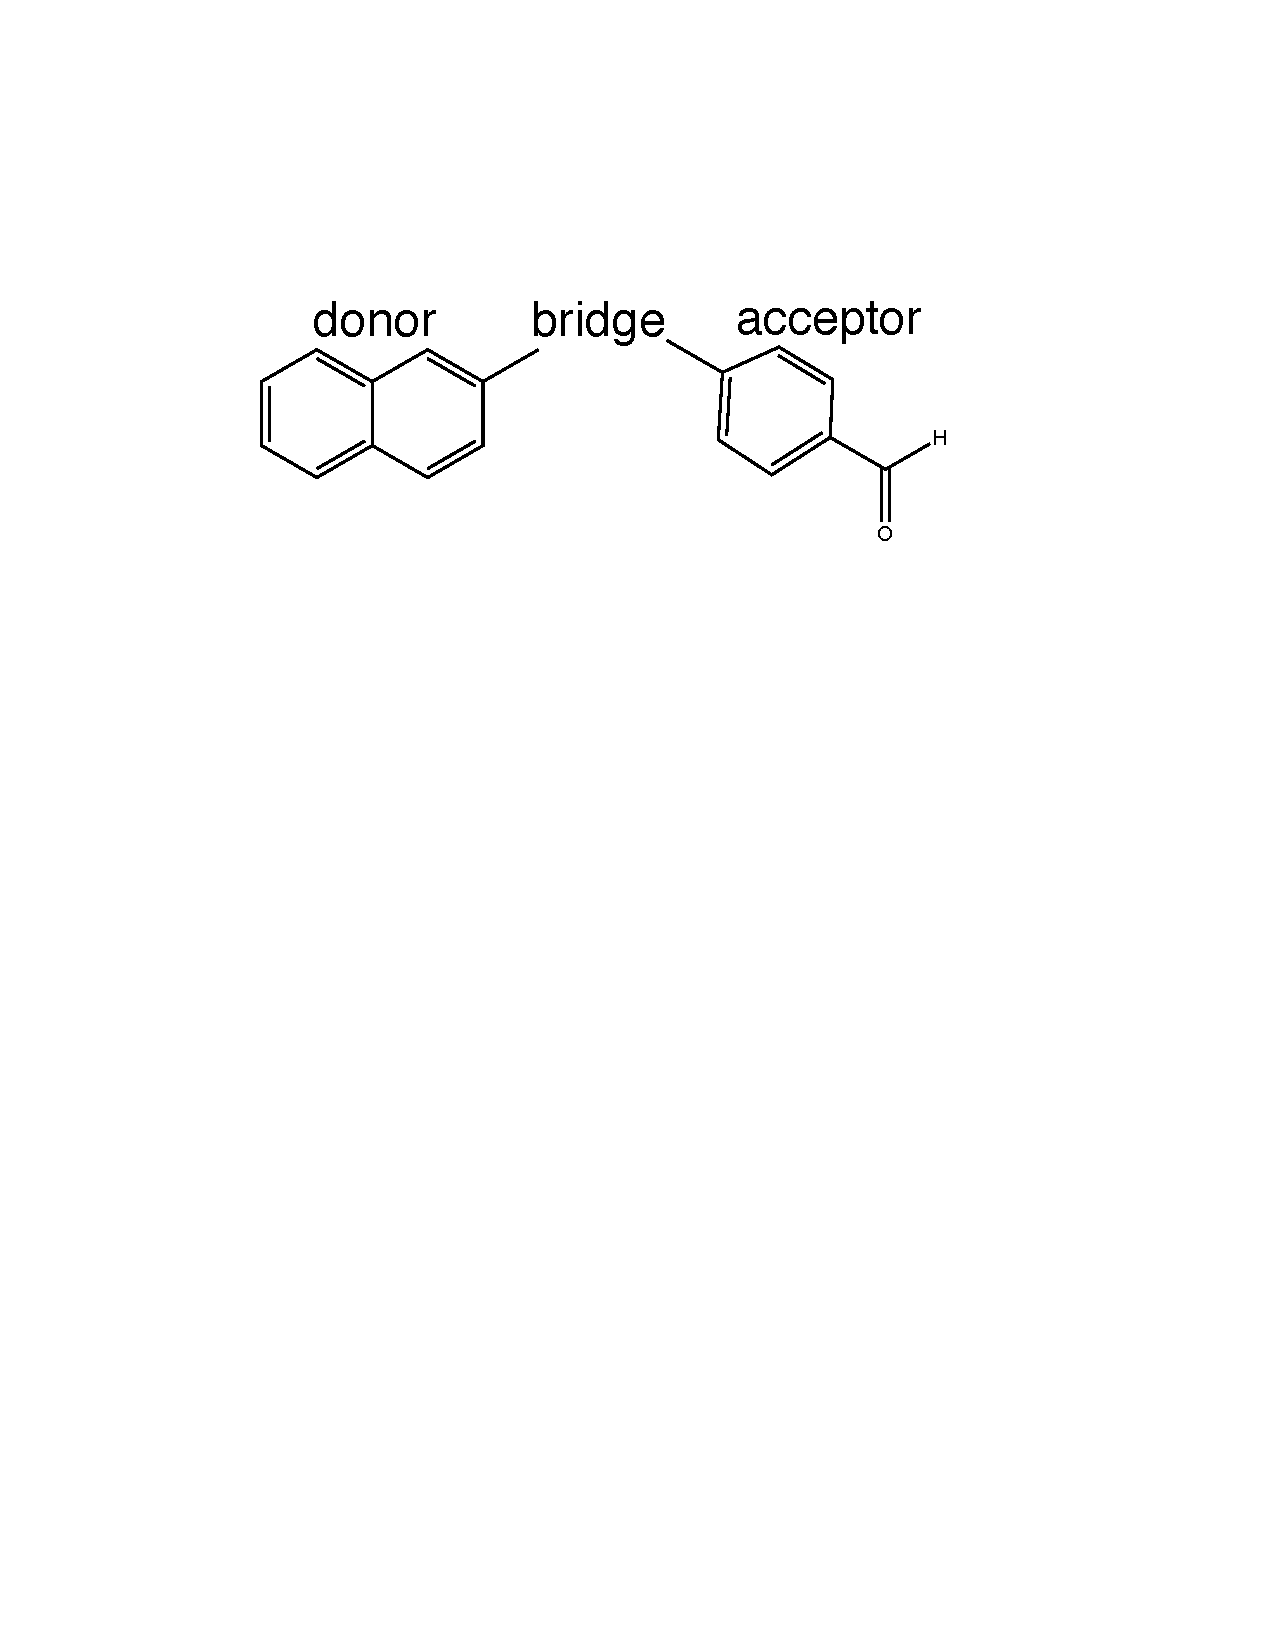
\includegraphics[height=1.5cm]{Chapters/chap2/Scheme1}
\end{table}

\lyxframeend{}




\lyxframeend{}\lyxframe{Benchmark with Closs' Experiments (Cont'd)}


\begin{figure}


\begin{centering}
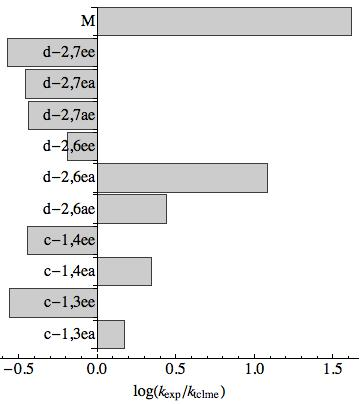
\includegraphics[width=0.5\textwidth]{Chapters/chap2/Figure3}
\caption{Comparison between predicted (TCLME) rate constants and the experimental rates.  With exception of
the methyl bridged and d-2,6ea cases, the TCLME results are in good agreement with the experimental results.  }\label{compare}
\par\end{centering}

\end{figure}

\lyxframeend{}


\lyxframeend{}\lyxframe{Why TCLME}
\begin{itemize}
\item Marcus theory
\end{itemize}
\[
H=\hat{T}_{n}+\left(\begin{array}{cc}
\epsilon_{a}(\mathbf{R}) & V_{ab}\\
V_{ab} & \epsilon_{b}(\mathbf{R})
\end{array}\right)
\]


\[
k=\frac{2\pi}{\hbar}|V_{ab}|^{2}\frac{1}{\sqrt{4\text{\ensuremath{\pi}}k_{B}T\lambda}}e^{-(\lambda+\Delta E)^{2}/4\text{\ensuremath{\lambda}}k_{B}T}
\]

\begin{itemize}
\item TCLME
\end{itemize}
% \[
% H_{dia}=\left(\begin{array}{cc}
% \epsilon_{a} & V_{ab}\\
% V_{ab} & \epsilon_{b}
% \end{array}\right)+\left(\begin{array}{cc}
% \\
%  & \sum_{i}g_{22i}q_{i}
% \end{array}\right)+h.o.
% \]


\[
H=\left(\begin{array}{cc}
E_{a}\\
 & E_{b}
\end{array}\right)+\sum_{ijq}g_{ijq}|\phi_{i}\rangle\langle\phi_{j}|q+\sum_{q}\hbar\omega_{q}(n+1/2)
\]
\[
H=\left(\begin{array}{cc}
E_{a}\\
 & E_{b}
\end{array}\right)+\left(\begin{array}{cc}
\sin^{2}\theta & \frac{1}{2}\sin2\theta\\
\frac{1}{2}\sin2\theta & \cos^{2}\theta
\end{array}\right)\sum_{i=1}^{NMode}g_{22i}q_{i}+h.o.
\]

% Advantages
% \begin{itemize}
% \item Go beyond Condon approximation easily
% \item Treat normal modes explicitly, which makes projection approach applicable
% \end{itemize}
TCLME treats normal modes explicitly, which makes projection approach applicable.
\lyxframeend{}


\lyxframeend{}\lyxframe{Projected Modes}

\[
H=\left(\begin{array}{cc}
E_{a}\\
 & E_{b}
\end{array}\right)+\left(\begin{array}{cc}
\sum_{i}g_{11i}q_{i} & \sum_{i}g_{12i}q_{i}\\
\sum_{i}g_{12i}q_{i} & \sum_{i}g_{22i}q_{i}
\end{array}\right)+\sum_{i}\frac{p_{i}^{2}}{2}+\frac{1}{2}\mathbf{q}^{T}\Omega\mathbf{q},
\]
where
\[
\mathbf{q}^{T}=\left(q_{1},q_{2},\cdots,q_{n}\right),\Omega=\left(\begin{array}{cccc}
\omega_{1}^{2}\\
 & \omega_{2}^{2}\\
 &  & \ddots\\
 &  &  & \omega_{n}^{2}
\end{array}\right)
\]
can be transformed to
\[
\Omega'=\left(\begin{array}{cccccc}
\omega_{1}'^{2} &  &  & \gamma_{14} & \cdots & \gamma_{1n}\\
 & \omega_{2}'^{2} &  & \gamma_{24} & \cdots & \gamma_{2n}\\
 &  & \omega_{3}'^{2} & \gamma_{34} & \cdots & \gamma_{3n}\\
\gamma_{14} & \gamma_{24} & \gamma_{24} & \omega_{4}'^{2}\\
\vdots & \vdots & \vdots &  & \ddots\\
\gamma_{1n} & \gamma_{2n} & \gamma_{3n} &  &  & \omega_{n}'^{2}
\end{array}\right)
\]



\lyxframeend{}



\lyxframeend{}\lyxframe{TCLME Equation}

\[
\frac{dP_{n}}{dt} = \sum_{m \ne n} W_{nm}(t)P_{m}(t) - \sum_{m \ne n} W_{mn}(t)P_{n}(t)
\]
\[
W_{nm}(t)=2{\rm Re}\int_{0}^{t} \! \mathrm{d}\tau \left\langle \hat V_{nm}(0)\hat V_{mn}\left(\tau\right)\right\rangle e^{-i(\tilde\epsilon_m - \tilde\epsilon_n)\tau}\]
The renormalization energy is
\[
\tilde\epsilon_n=\epsilon_n-\sum_{i}\frac{g_{nni}^2}{\hbar\omega_i}\]

$\left\langle \hat V_{nm}(0)\hat V_{mn}\left(\tau\right)\right\rangle$ is the correlation function.
\lyxframeend{}


\lyxframeend{}\lyxframe{Projected Modes for c-1,4ee and d-2,6ae}
\begin{figure}[t]
\subfloat{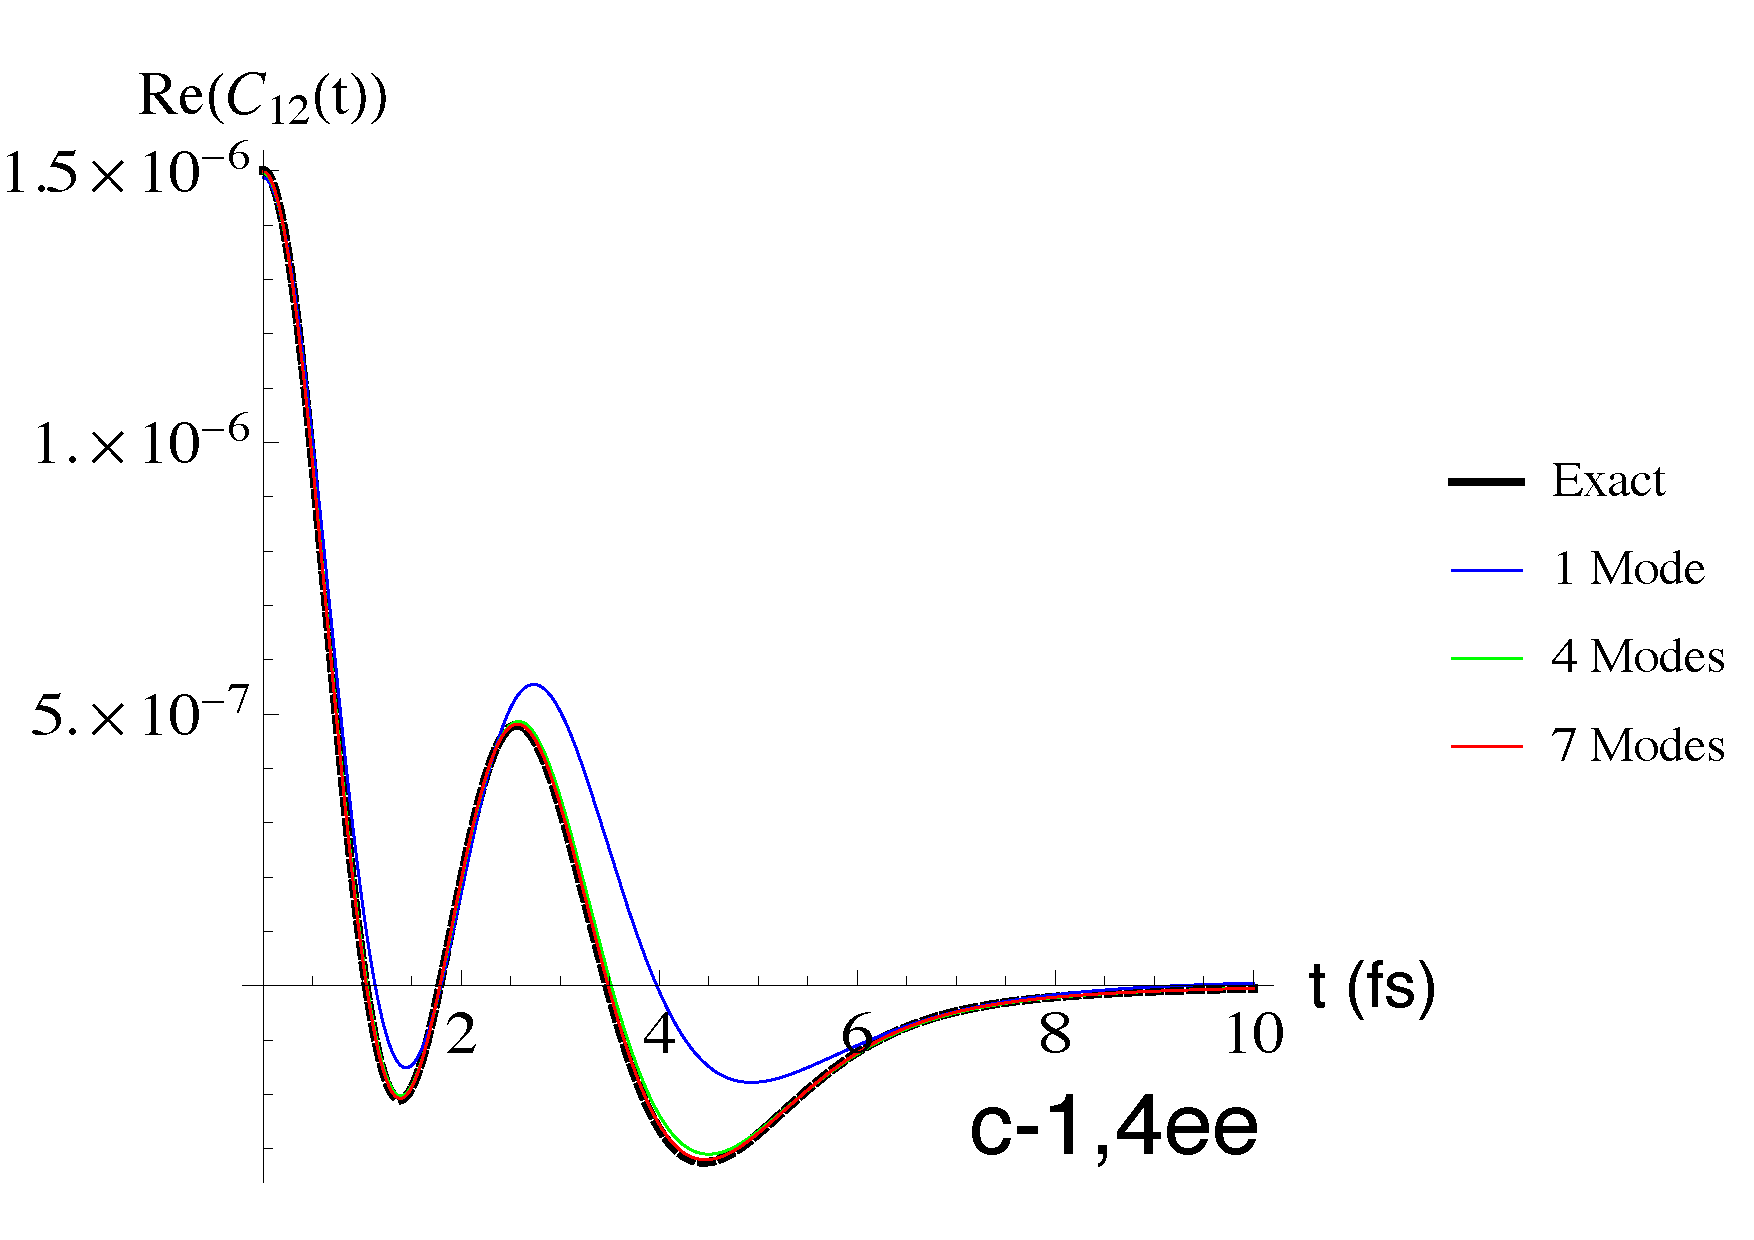
\includegraphics[width=0.5\columnwidth]{Chapters/chap2/Figure5a}}
\subfloat{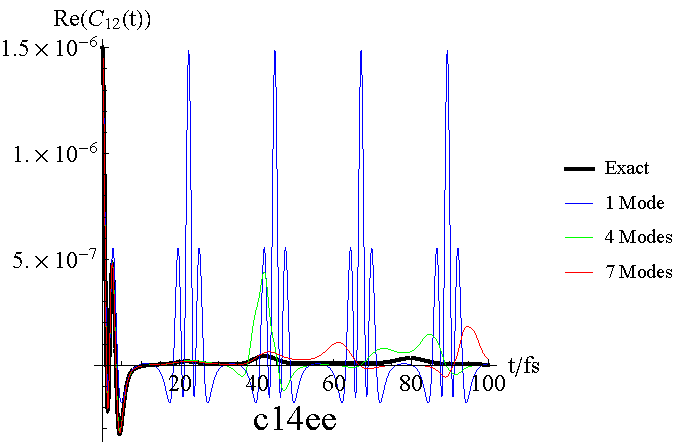
\includegraphics[width=0.5\columnwidth]{Chapters/chap2/Figure5b}}\\
\subfloat{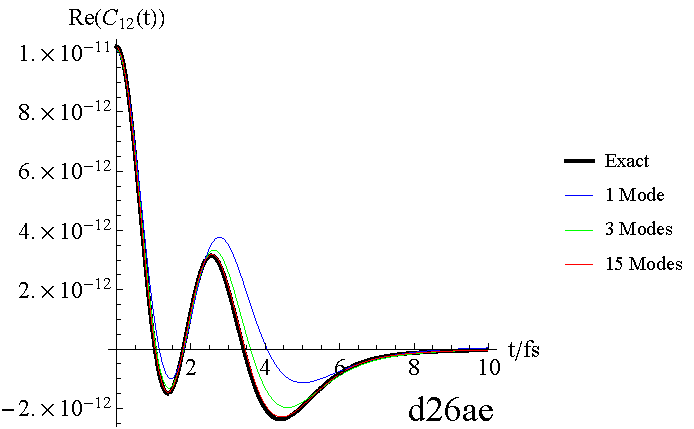
\includegraphics[width=0.5\columnwidth]{Chapters/chap2/Figure5c}}
\subfloat{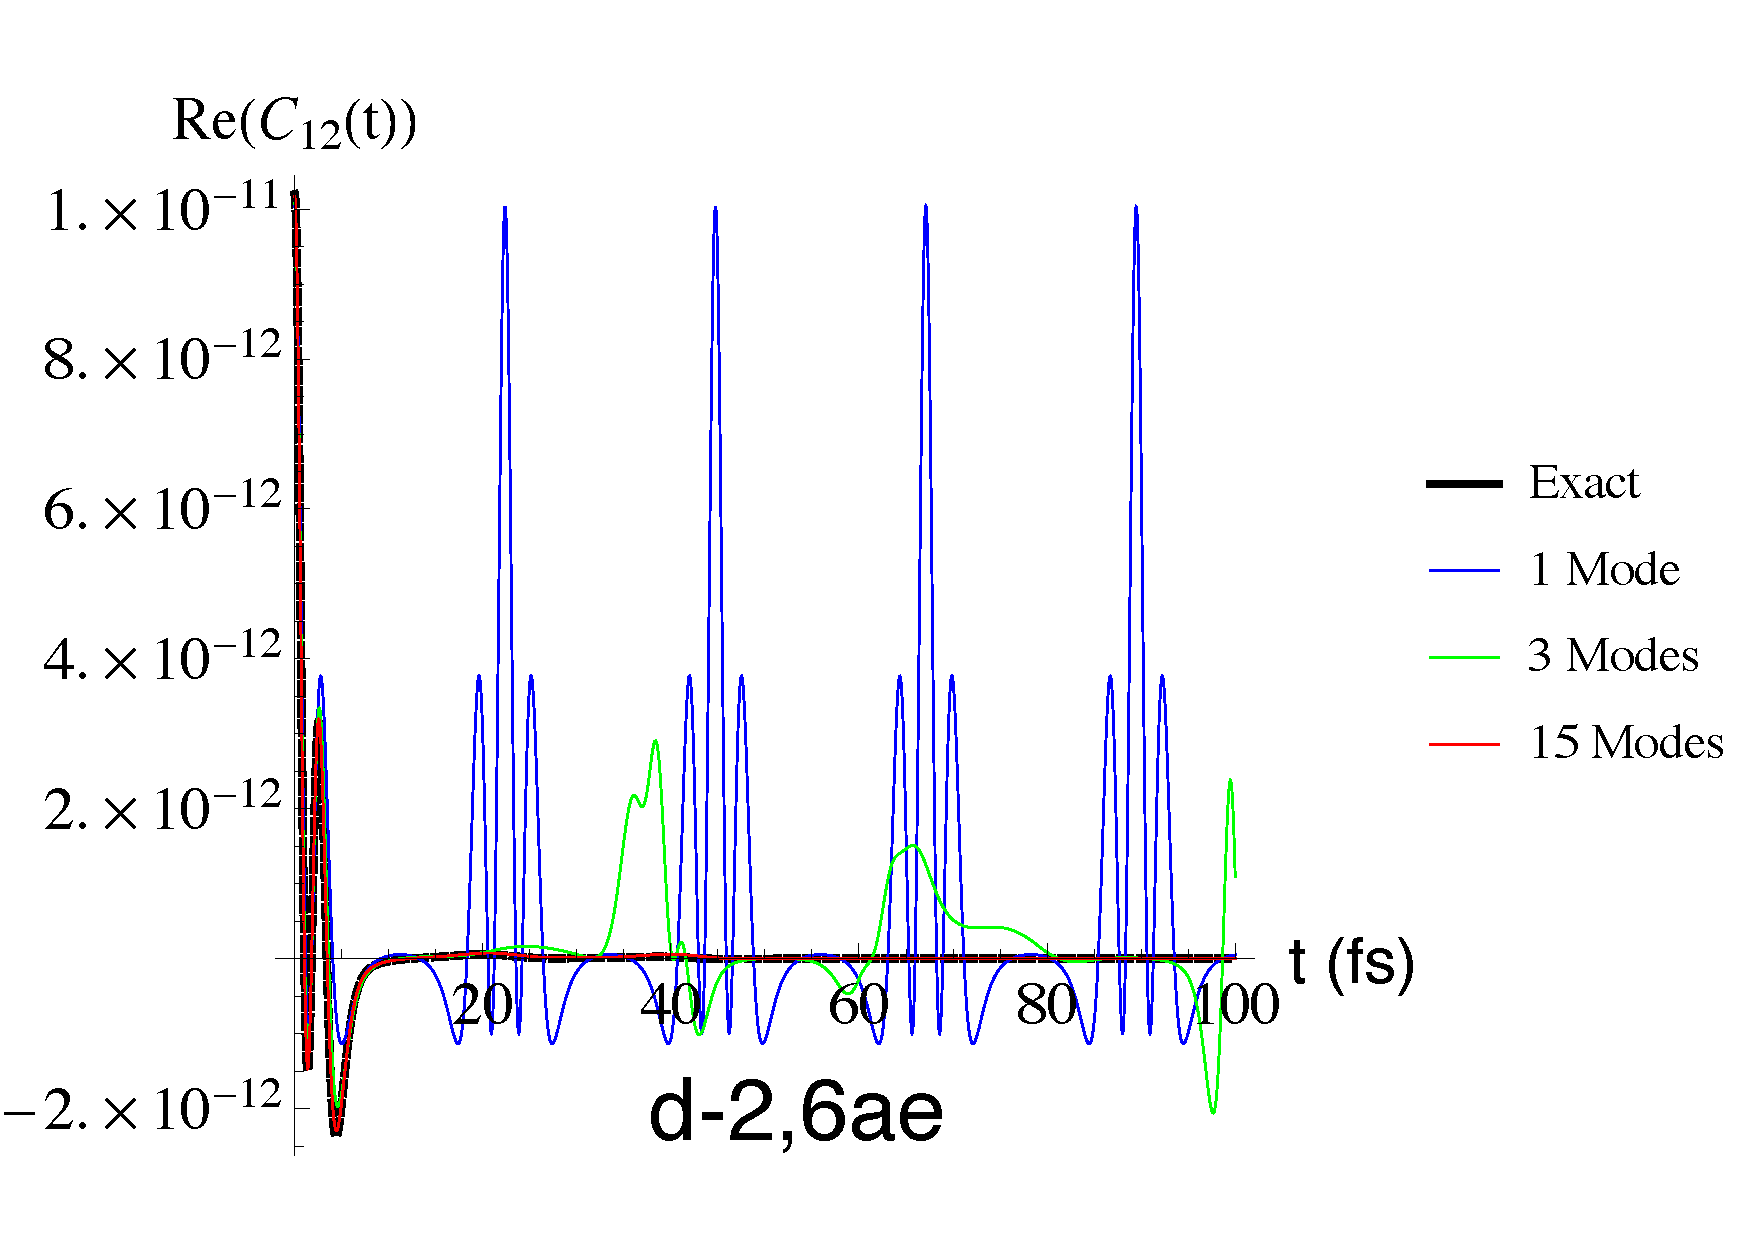
\includegraphics[width=0.5\columnwidth]{Chapters/chap2/Figure5d}}
% \caption{Convergence of the electronic coupling autocorrelation function (Eq. ~\ref{c-of-t})
% with respect to number of reduced modes.\label{firstmodecorr}}
\end{figure}


\lyxframeend{}




\lyxframeend{}\lyxframe{Primary Mode Rate Constant}

\[
\frac{dP_{n}}{dt} = \sum_{m \ne n} W_{nm}(t)P_{m}(t) - \sum_{m \ne n} W_{mn}(t)P_{n}(t)
\]
\[
W_{nm}(t)=2{\rm Re}\int_{0}^{t} \! \mathrm{d}\tau \left\langle \hat V_{nm}(0)\hat V_{mn}\left(\tau\right)\right\rangle e^{-i(\tilde\epsilon_m - \tilde\epsilon_n)\tau}\]
\[
\tilde\epsilon_n=\epsilon_n-\sum_{i}\frac{g_{nni}^2}{\hbar\omega_i}\]

\begin{itemize}
\item How about using the approximated correlation function and $\Delta\epsilon$ to calculate the rate?
\item How about the approximated correlation function with exact $\Delta\epsilon$?
\end{itemize}

\lyxframeend{}




\lyxframeend{}\lyxframe{Primary Mode Rate Constant (Cont'd)}
\begin{figure}[t]
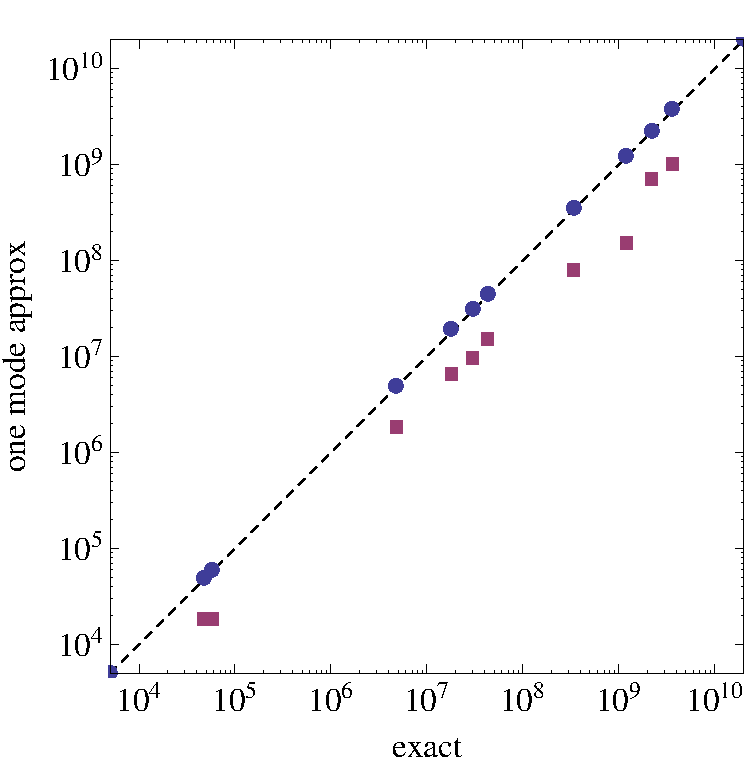
\includegraphics[width=0.45\columnwidth]{Chapters/chap2/Figure6}
\caption{Comparison between exact rate constant and its primary mode approximation.  The blue dots correspond to rates computed using
only the primary mode and the renormalized energy for only that mode.  The red points use the primary mode and the exact
renormalized energies. }\label{fig-1mode}
\end{figure}

Only one mode? Seems easy. Any other way possible?
\lyxframeend{}




\lyxframeend{}\lyxframe{No Normal Mode Works That Well}
\begin{table}[t]
\centering
\begin{tabular}{lrrr}
 bridge   &  $\omega_1$(eV)  & $|g_{1}|$ (eV)  &  $|g_{max}|$ (eV)  \\
\hline
\hline
 c-1,3ea  &           0.184  &         0.367  &           0.159  \\
 c-1,3ee  &           0.185  &         0.365  &           0.162  \\
 c-1,4ea  &           0.185  &         0.367  &           0.166  \\
 c-1,4ee  &           0.185  &         0.370  &           0.171  \\
 d-2,6ae  &           0.185  &         0.367  &           0.159  \\
 d-2,6ea  &           0.185  &         0.367  &           0.142  \\
 d-2,6ee  &           0.185  &         0.365  &           0.143  \\
 d-2,7ae  &           0.184  &         0.366  &           0.165  \\
 d-2,7ea  &           0.185  &         0.367  &           0.142  \\
 d-2,7ee  &           0.185  &         0.370  &           0.149  \\
 M           &           0.184  &         0.366  &           0.160  \\
 \hline
\end{tabular}
\caption{Frequencies and dimensionless electron-phonon couplings for
the primary mode. The last column gives the
absolute value of the largest coupling constant within the normal mode basis.
}
\end{table}
$|g_1|$ is more than twice of the largest $|g_i|$. No single normal mod is as representative as the primary mode. Actually, the primary mode generates the largest possible coupling constant.
\lyxframeend{}


\lyxframeend{}\lyxframe{Primary Mode}

\begin{figure}
\subfloat[c-1,4ee: $\omega=1492.47cm^{-1},g=0.370eV$]{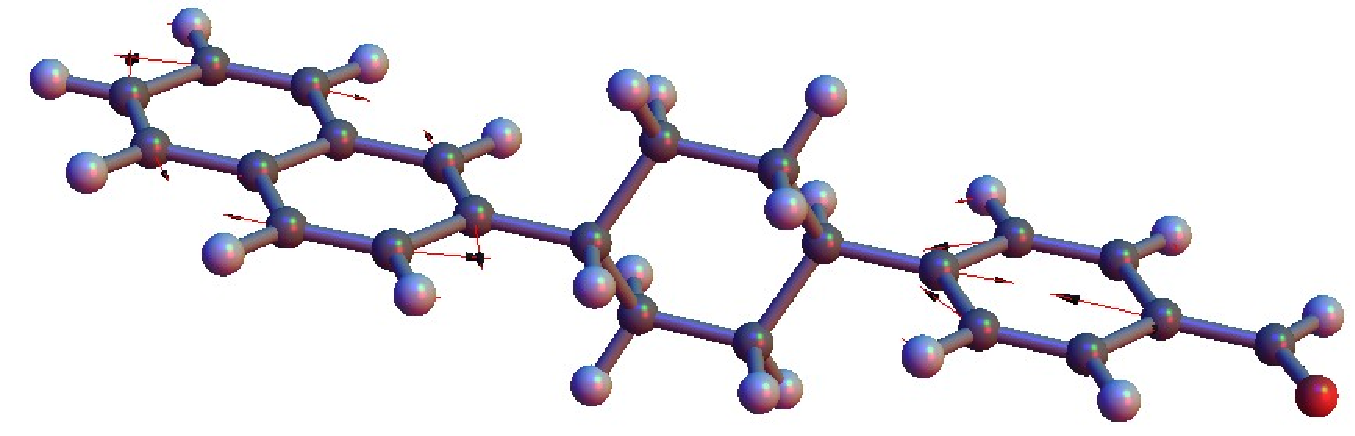
\includegraphics[width=0.55\columnwidth]{Chapters/chap2/Figure4a}}\\
\subfloat[d-2,6ae $\omega=1491.09cm^{-1},g=0.367eV$]{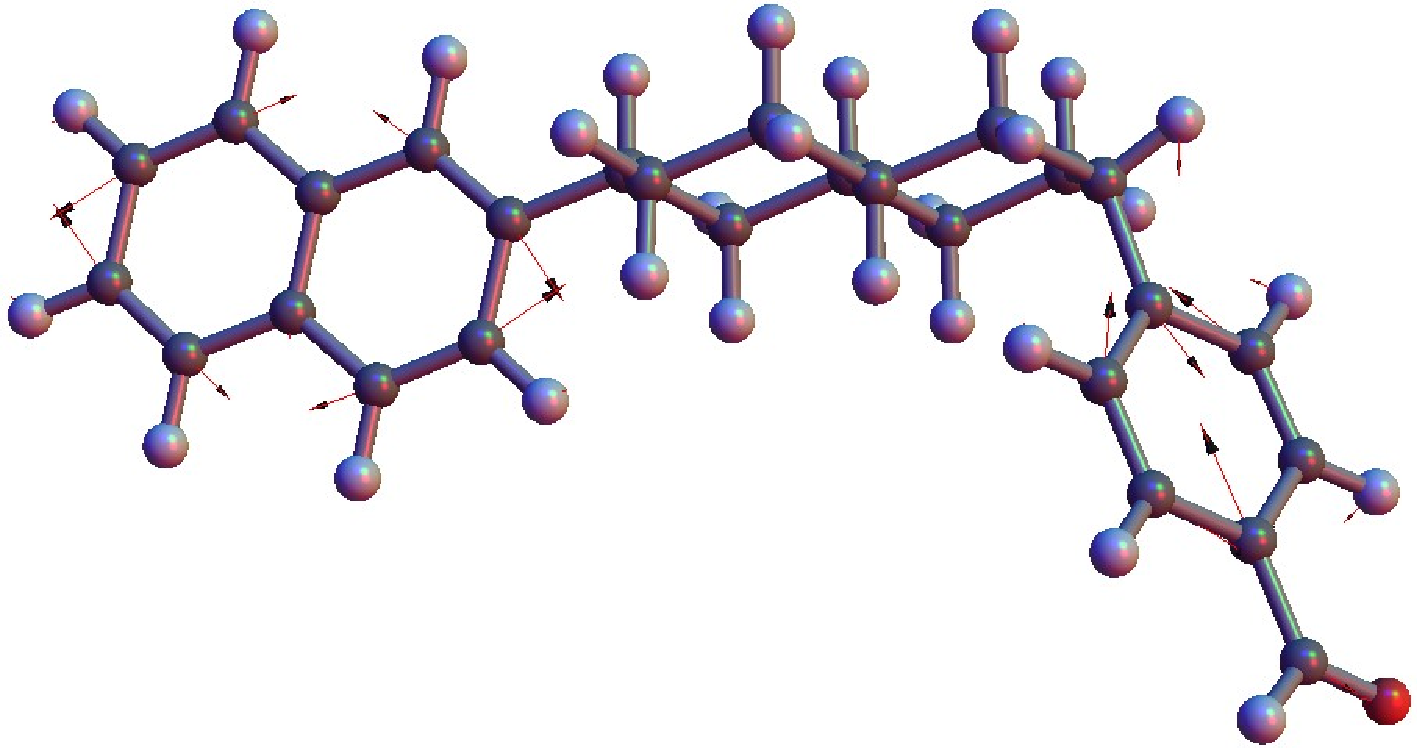
\includegraphics[width=0.55\columnwidth]{Chapters/chap2/Figure4b}}
\end{figure}
\begin{itemize}
\item Bridge is barely involved
\item Certain local symmetry
\end{itemize}
\lyxframeend{}



\lyxframeend{}\lyxframe{Phenyl and Anthracene as Acceptors}

\begin{figure}[t]
\subfloat{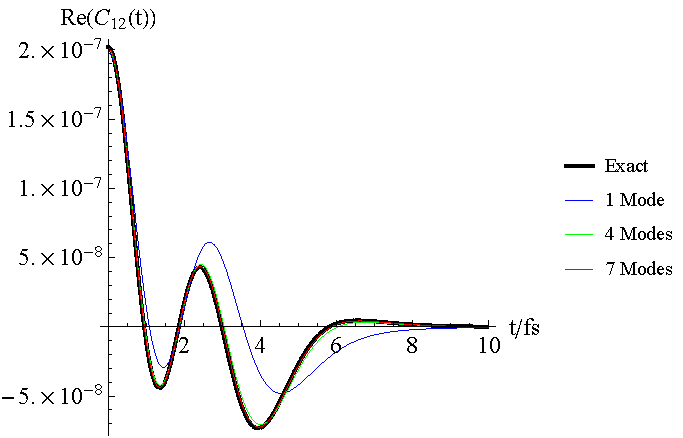
\includegraphics[width=0.49\columnwidth]{Chapters/chap3/Figure3a.pdf}}
\subfloat{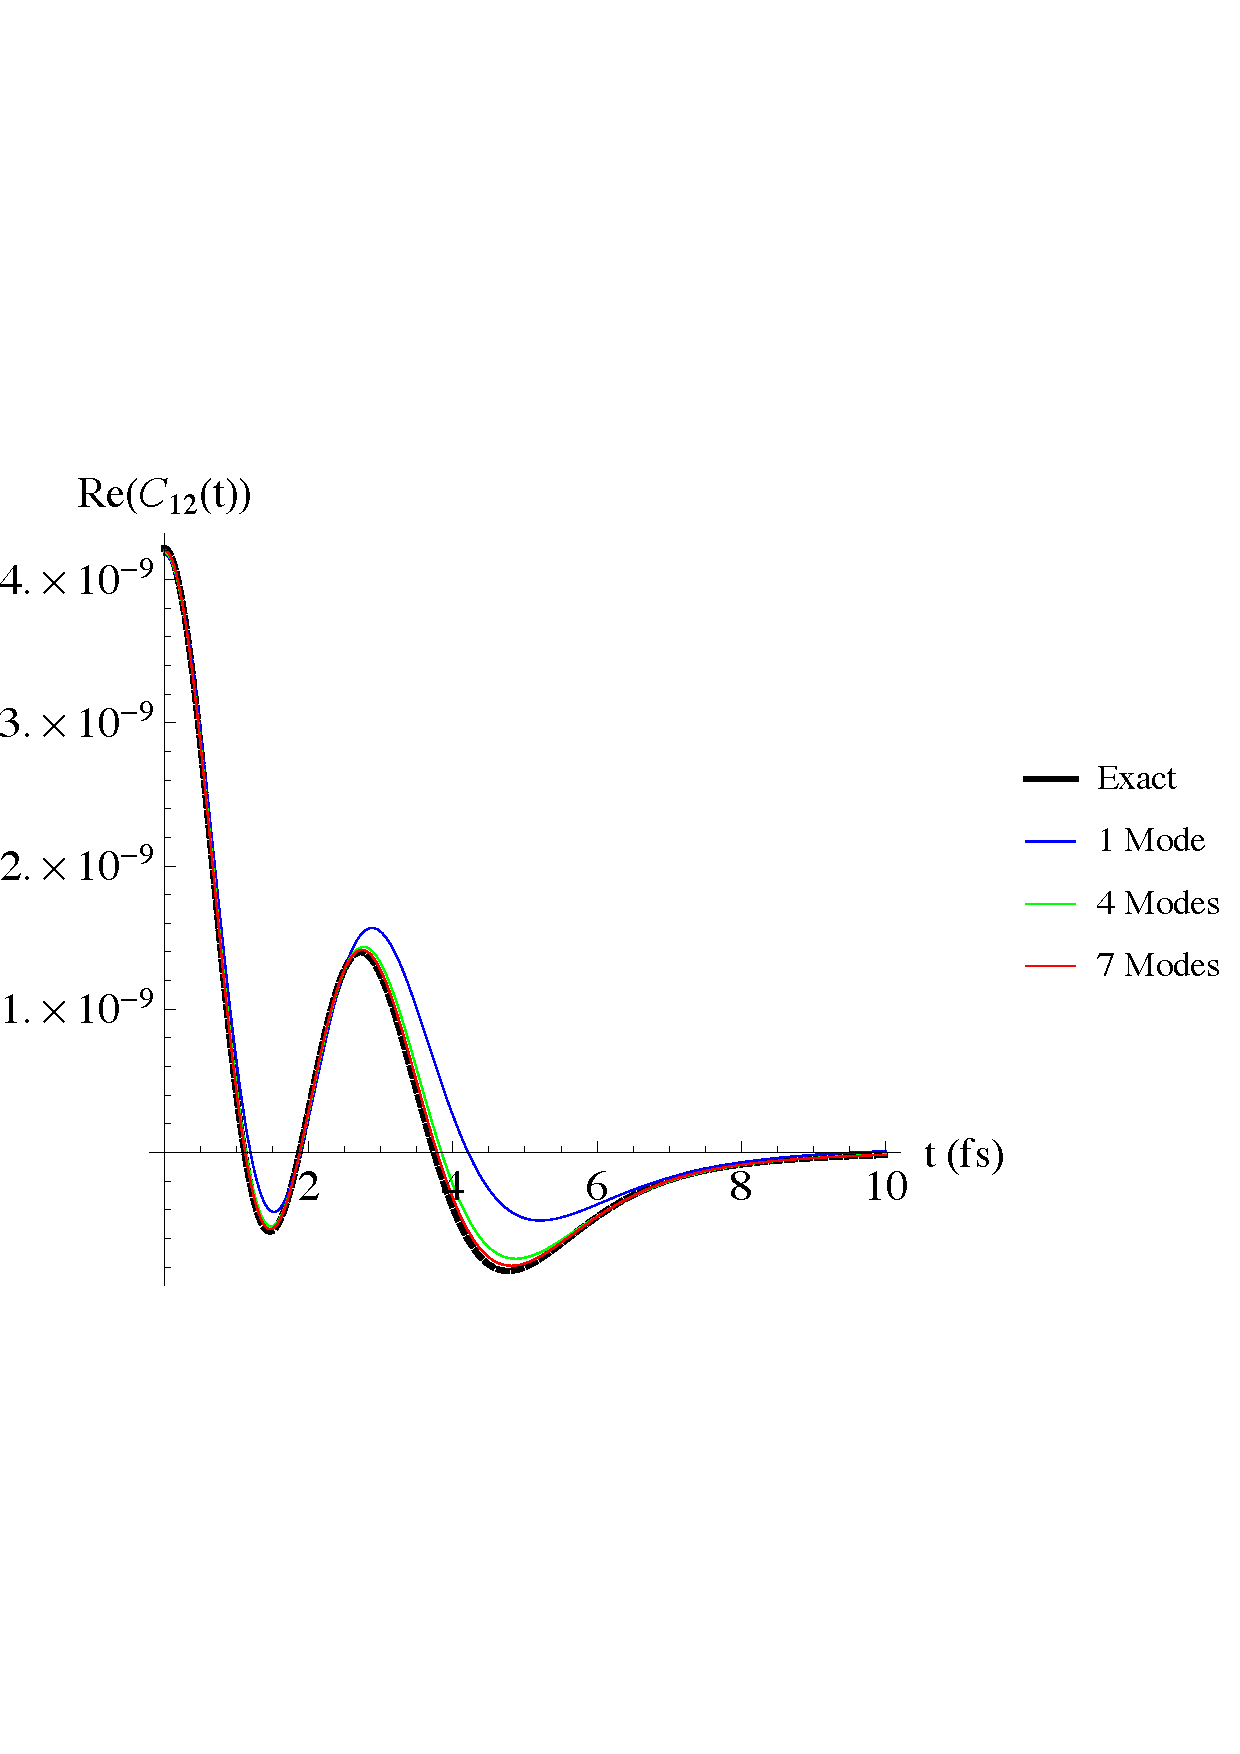
\includegraphics[width=0.49\columnwidth]{Chapters/chap3/Figure3b.pdf}}\\
\subfloat{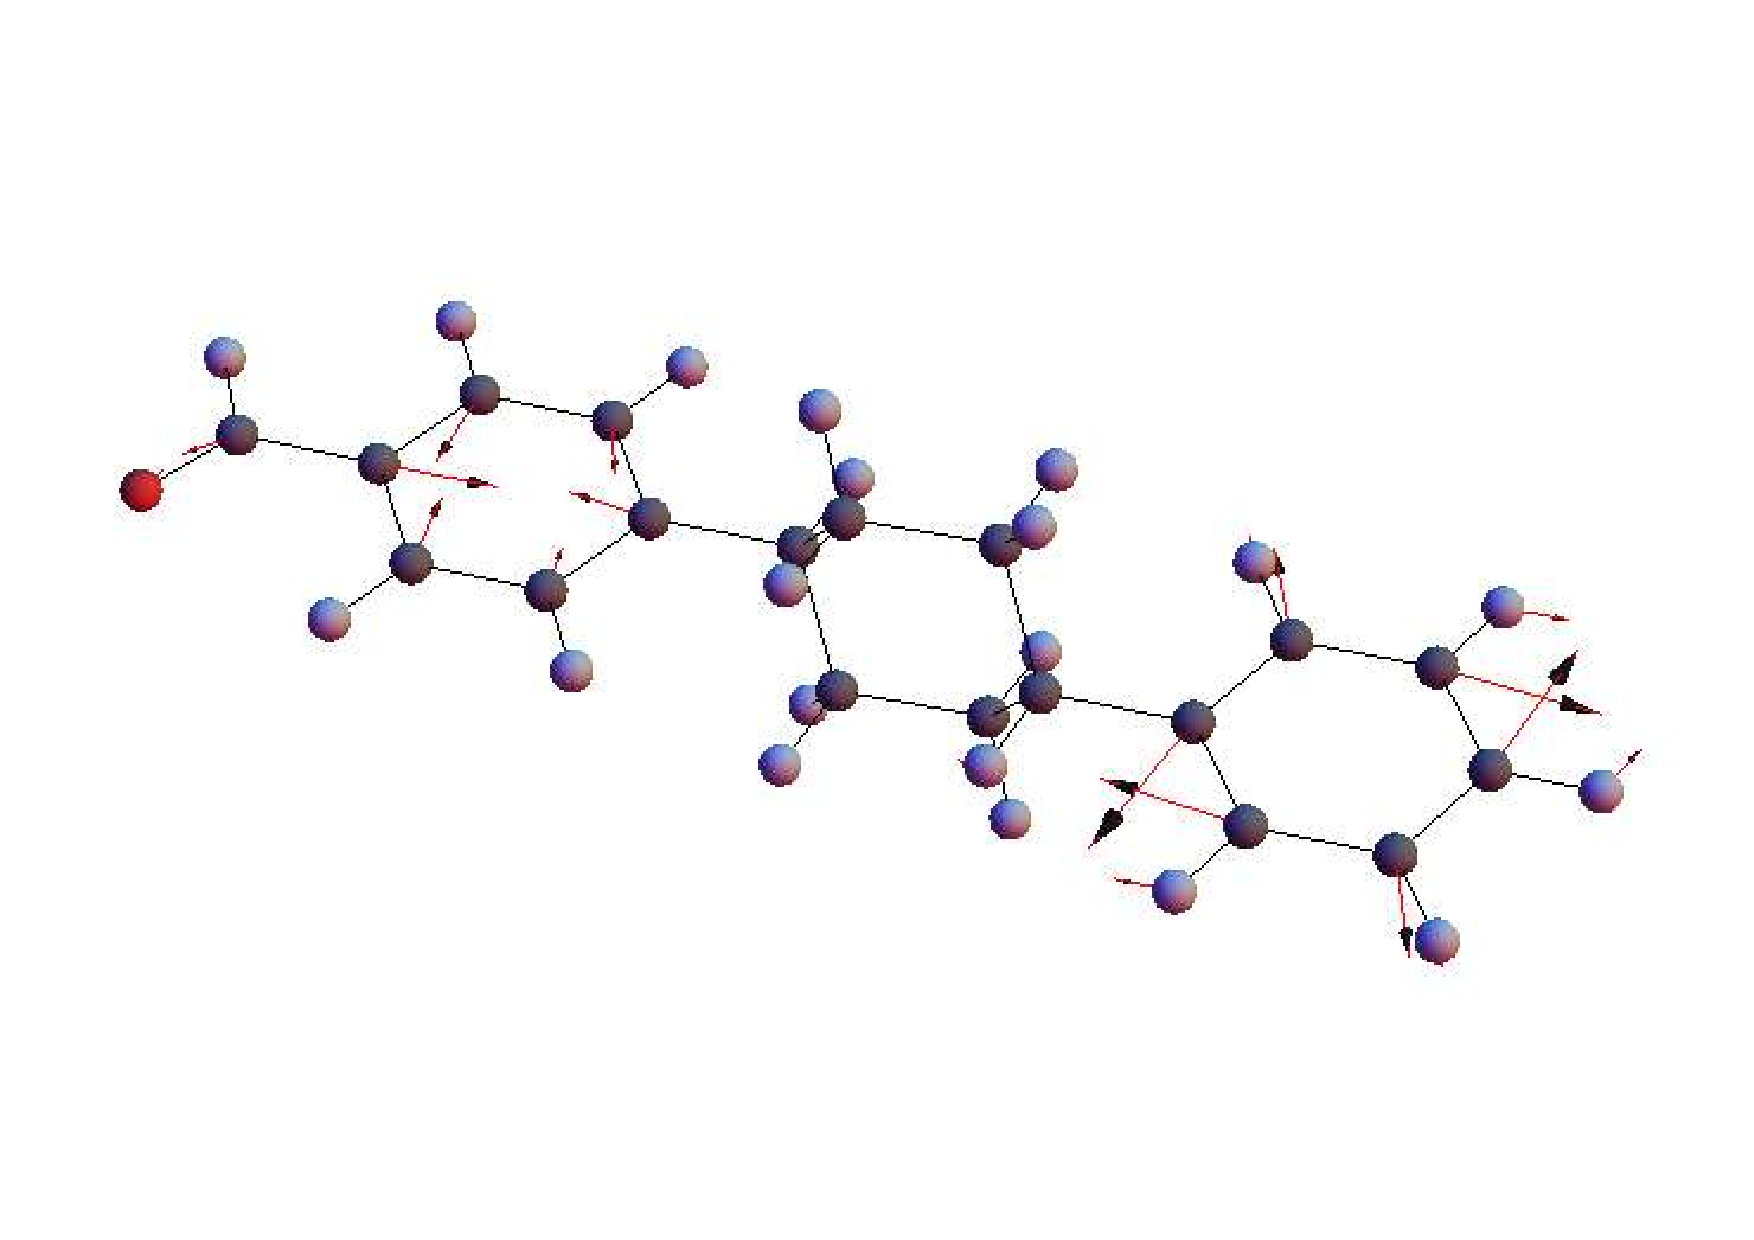
\includegraphics[width=0.49\columnwidth]{Chapters/chap3/Figure3c.pdf}}
\subfloat{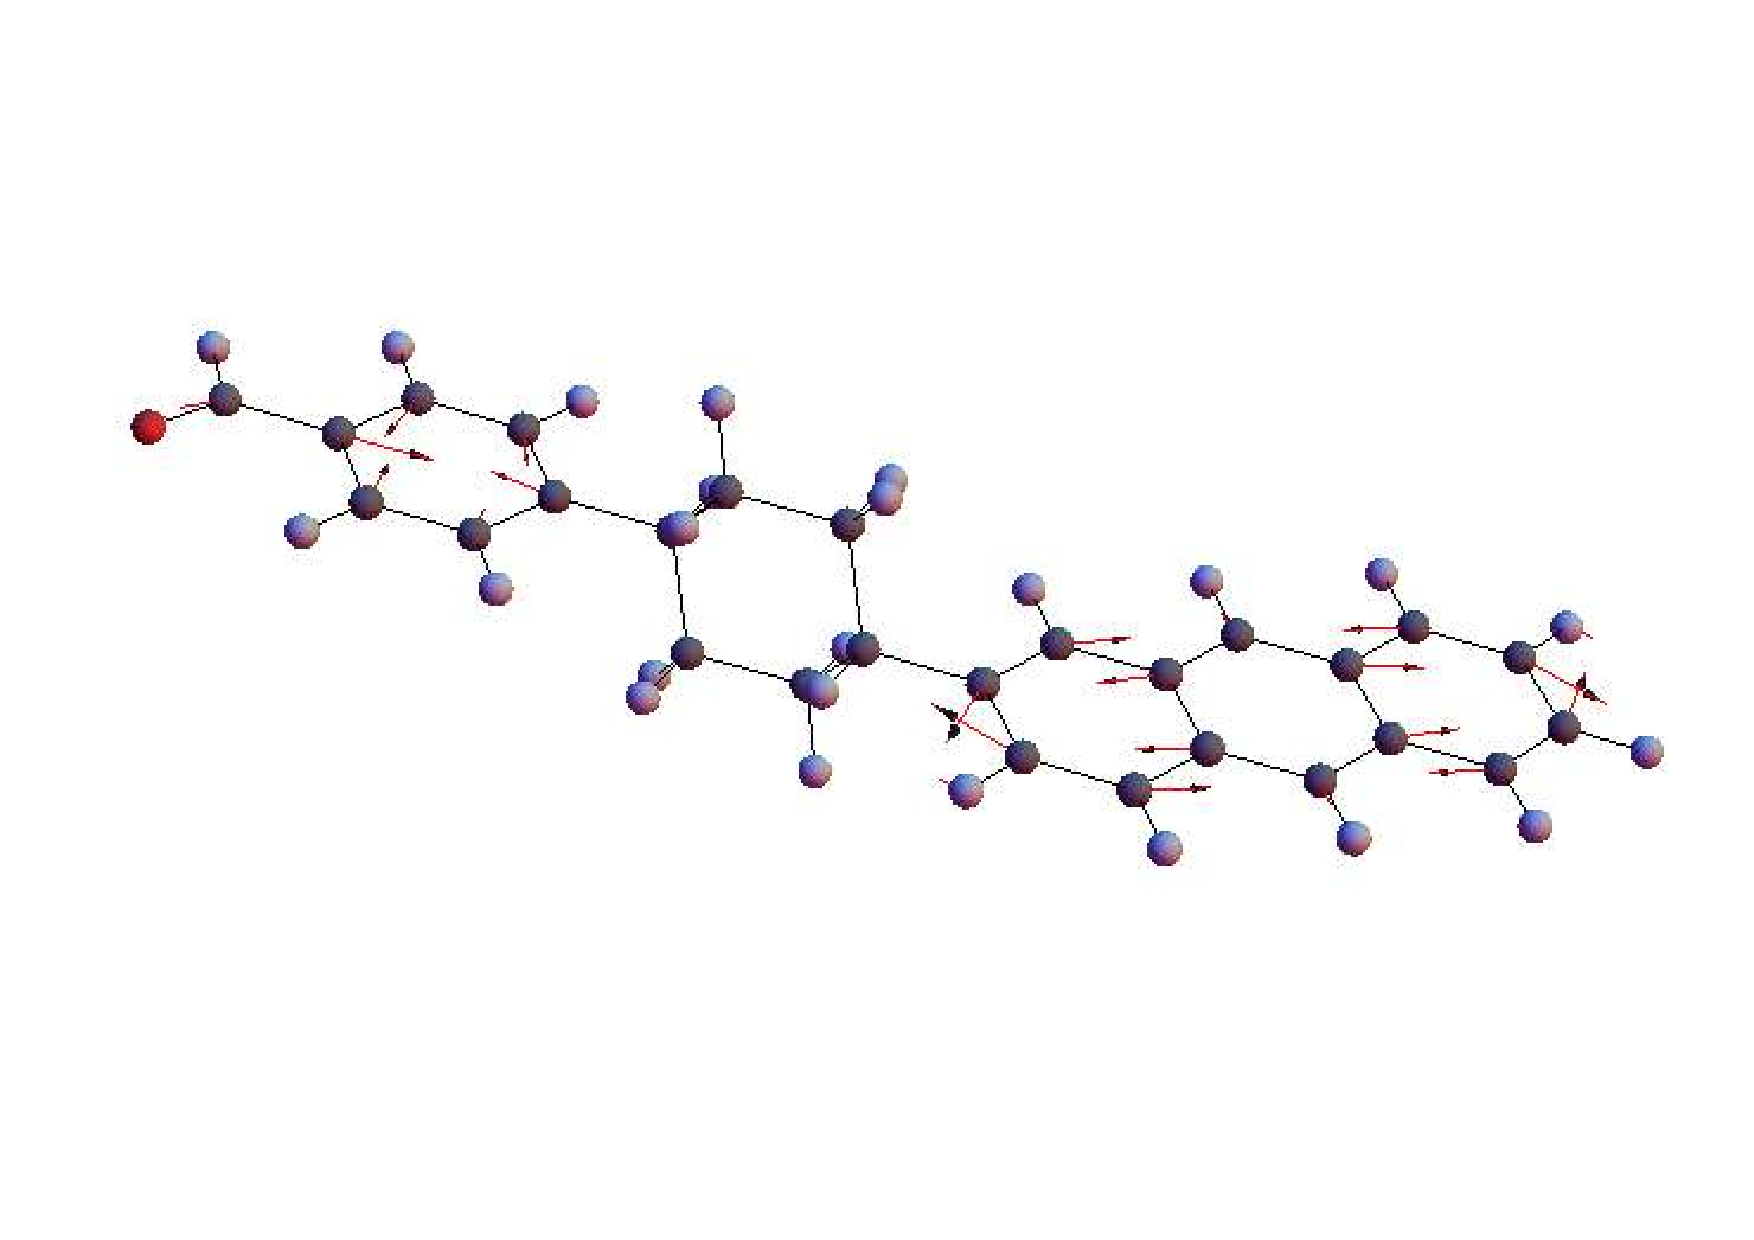
\includegraphics[width=0.49\columnwidth]{Chapters/chap3/Figure3d.pdf}}
\end{figure}


\lyxframeend{}



\lyxframeend{}\lyxframe{Projection on Moiety}

\begin{figure}[ht]
\subfloat[]{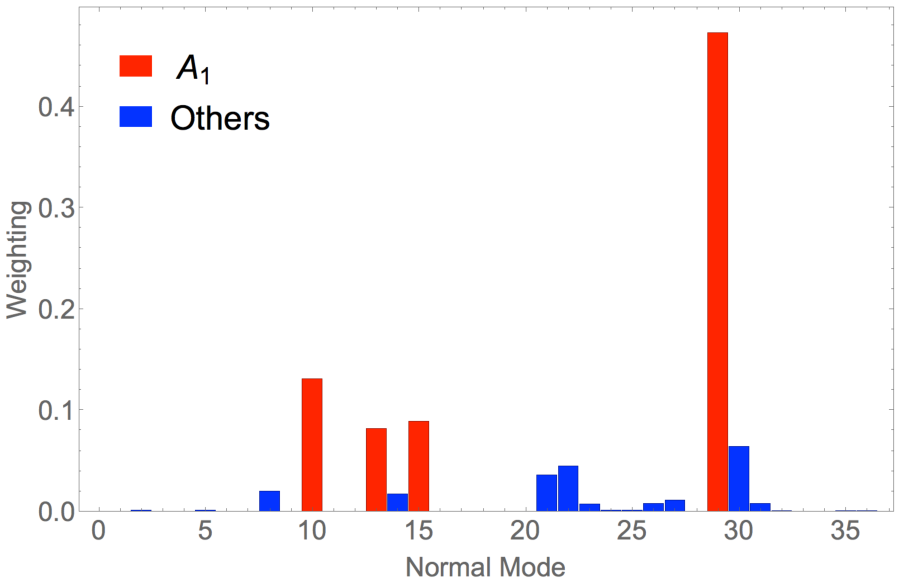
\includegraphics[width=0.38\columnwidth]{Chapters/chap3/Figure2a.pdf}}
\subfloat[]{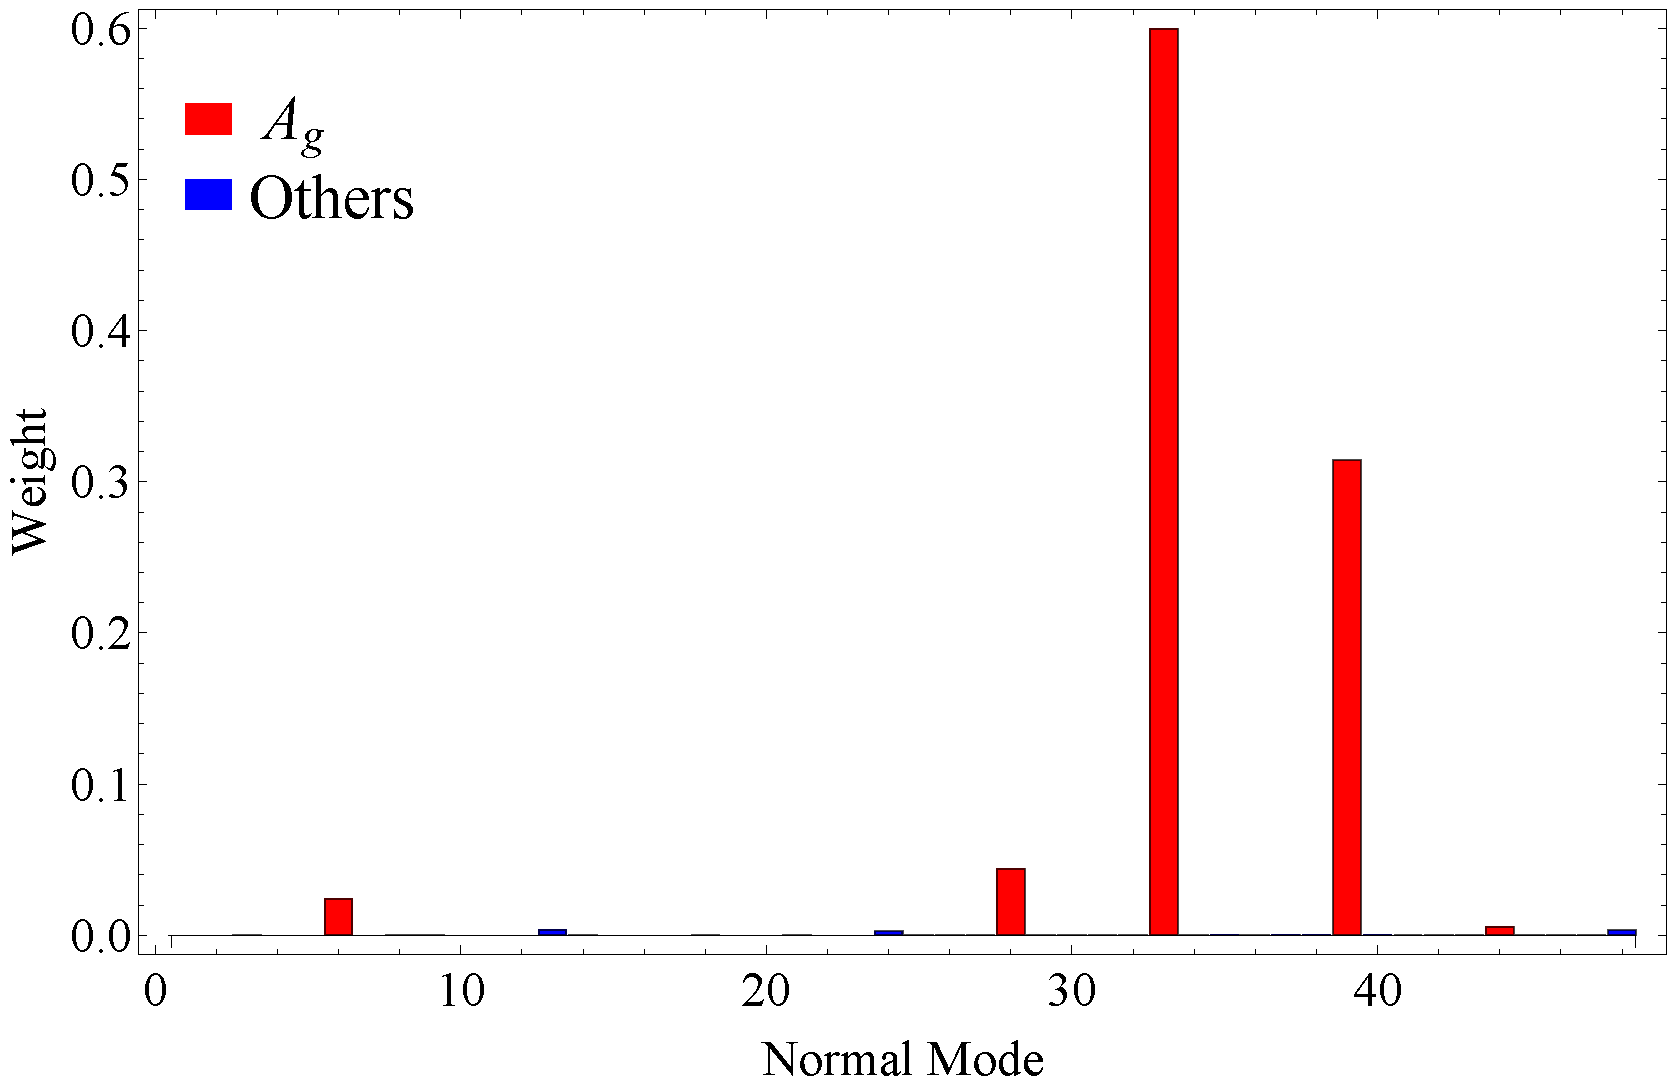
\includegraphics[width=0.38\columnwidth]{Chapters/chap3/Figure2b.pdf}} \\
\subfloat[]{\includegraphics[width=0.38\columnwidth]{Chapters/chap3/Figure2c.pdf}}
\subfloat[]{\includegraphics[width=0.38\columnwidth]{Chapters/chap3/Figure2d.pdf}}
\caption{Projection on (a) benzaldehyde, (b) symmetrized naphthalene in c-1,4ee, (c) benzaldehyde, (d) symmetrized naphthalene in d-2,6ae. \label{fragProj}}
\end{figure}


\lyxframeend{}

\lyxframeend{}\lyxframe{Bridge Is Not Important}

\begin{figure}[!h]
\subfloat{\includegraphics[width=0.33\columnwidth]{Chapters/chap3/Figure7a.pdf}}
\subfloat{\includegraphics[width=0.33\columnwidth]{Chapters/chap3/Figure7b.pdf}} \\
\subfloat{\includegraphics[width=0.33\columnwidth]{Chapters/chap3/Figure7c.pdf}}
\subfloat{\includegraphics[width=0.33\columnwidth]{Chapters/chap3/Figure7d.pdf}}
\caption{``Exact'' = primary mode.  ``NfBf" = all normal modes of D and A.
``NxBy'' = $x$ most significant normal modes
on naphthalene + $y$ most significant ones on benzaldehyde. (c) and (d):
 relative error in rate constants compared to the exact result
 of c-1,4ee (c) and d-2,6ae (d), respectively. \label{backCorr}}
\end{figure}
\lyxframeend{}



\lyxframeend{}\lyxframe{Primary Mode and Electron Orbital}

\begin{figure}[t]
\subfloat{\includegraphics[width=0.65\columnwidth]{Chapters/chap2/Figure4b}}\\
\subfloat[HOMO]{\includegraphics[width=0.4\columnwidth]{Chapters/chap3/Figure4a.pdf}}
\subfloat[LUMO]{\includegraphics[width=0.4\columnwidth]{Chapters/chap3/Figure4b.pdf}}
\end{figure}


\lyxframeend{}

\lyxframeend{}\lyxframe{Geometry Change On Benzaldehyde}

\begin{figure}[t]
\subfloat[Geometry change]{\includegraphics[width=0.4\columnwidth]{Chapters/chap3/Figure8a.pdf}
\includegraphics[width=0.4\columnwidth]{Chapters/chap3/Figure8c.pdf}}\\
\subfloat[Primary mode]{\includegraphics[width=0.4\columnwidth]{Chapters/chap3/Figure2a.pdf}
\includegraphics[width=0.4\columnwidth]{Chapters/chap3/Figure2c.pdf}}
\end{figure}


\lyxframeend{}

\lyxframeend{}\lyxframe{Geometry Change On Naphthalene}

\begin{figure}[t]
\subfloat[Geometry change]{\includegraphics[width=0.4\columnwidth]{Chapters/chap3/Figure8b.pdf}
\includegraphics[width=0.4\columnwidth]{Chapters/chap3/Figure8d.pdf}}\\
\subfloat[Primary mode]{\includegraphics[width=0.4\columnwidth]{Chapters/chap3/Figure6a.pdf}
\includegraphics[width=0.4\columnwidth]{Chapters/chap3/Figure6b.pdf}}
\end{figure}


\lyxframeend{}




\lyxframeend{}\lyxframe{Primary Mode and Geometry Change}

\begin{figure}[t]
\subfloat[Primary mode]{\includegraphics[width=0.4\columnwidth]{Chapters/chap3/Figure5a.pdf}
\includegraphics[width=0.4\columnwidth]{Chapters/chap3/Figure5b.pdf}}\\
\subfloat[Geometry change]{\includegraphics[width=0.4\columnwidth]{Chapters/chap3/Figure9a.pdf}
\includegraphics[width=0.4\columnwidth]{Chapters/chap3/Figure9b.pdf}}
\end{figure}


\lyxframeend{}


\lyxframeend{}\lyxframe{Relaxation Mode Doesn't Contribute to Rate}

\begin{figure}[t]
\subfloat{\includegraphics[width=0.48\columnwidth]{Chapters/chap3/Figure9a.pdf}}
\subfloat{\includegraphics[width=0.48\columnwidth]{Chapters/chap3/Figure9b.pdf}}\\
\subfloat{\includegraphics[width=0.48\columnwidth]{Chapters/chap3/Figure10a.pdf}}
\subfloat{\includegraphics[width=0.48\columnwidth]{Chapters/chap3/Figure10b.pdf}}
\label{Corr}
\end{figure}


\lyxframeend{}


\lyxframeend{}\lyxframe{Internal and Gross Motions}

\begin{figure}[t]
\subfloat{\includegraphics[width=0.4\columnwidth]{Chapters/chap3/Figure10c.pdf}}
\subfloat{\includegraphics[width=0.4\columnwidth]{Chapters/chap3/Figure4a.pdf}}
\label{Corr}
\end{figure}
\begin{table}
\centering
 \begin{tabular}{lll}
   \hline
              & Max. bond length    & Max. bond angle  \\
   Mode used  & difference (\AA)    & difference (rad) \\
   \hline
   c-1,4ee-PM   & 0.034 & 0.053  \\
   c-1,4ee-RM   & 0.160 & 0.075 \\
   d-2,6ae-PM   & 0.039 & 0.057  \\
   d-2,6ae-RM   & 0.283 & 0.135 \\
   \hline
\end{tabular}
\caption{Approximated geometry using the primary mode (PM) and the relaxation modes (RM) compared to acceptor states
}
\end{table}
\lyxframeend{}

% \lyxframeend{}\lyxframe{Energy Diagram}
% \begin{figure}[!t]
% \includegraphics[width=\columnwidth]{Chapters/chap4/Images/molecules.jpg}
% % \includegraphics[width=0.4\columnwidth]{Chapters/chap4/Images/scheme.jpg}
% \caption{\textbf{a}. Molecular structure of PTZ-CH\textsubscript{2}-Pt-NAP, PTZ-Pt-NAP and OMe-PTZ-Pt-NAP, from left to right (D = PTZ is phenothiazine and A = NAP is naphthalene-monoimide). \textbf{b}. Energy level diagrams for the ET process, with the lifetimes and the driving force ($\Delta$G) of CT $\rightarrow$ CSS transfer  indicated. Adabtpe from Ref. \footnote{Delor, Milan, et al. ``On the mechanism of vibrational control of light-induced charge transfer in donor–bridge–acceptor assemblies.'' Nature chemistry (2015)}}
% \end{figure}

% \lyxframeend{}


\lyxframeend{}\lyxframe{Molecule Structure and Energy Diagram}

\begin{figure}[t]
\includegraphics[width=\columnwidth]{Chapters/chap4/Images/molecules.jpg}
\caption{\textbf{a}. Molecular structure of PTZ-CH\textsubscript{2}-Pt-NAP, PTZ-Pt-NAP and OMe-PTZ-Pt-NAP, from left to right (D = PTZ is phenothiazine and A = NAP is naphthalene-monoimide). \textbf{b}. Energy level diagrams for the ET process, with the lifetimes and the driving force ($\Delta$G) of CT $\rightarrow$ CSS transfer  indicated.}
\end{figure}
\small{Delor, Milan, et al. ``On the mechanism of vibrational control of light-induced charge transfer in donor–bridge–acceptor assemblies.'' Nature Chemistry (2015)}
\lyxframeend{}


\lyxframeend{}\lyxframe{IR Control Scheme}

\begin{figure}[t]
\includegraphics[width=0.65\columnwidth]{Chapters/chap4/Images/scheme.jpg}
\end{figure}
\small{Delor, Milan, et al. ``On the mechanism of vibrational control of light-induced charge transfer in donor–bridge–acceptor assemblies.'' Nature Chemistry (2015)}
\lyxframeend{}



\lyxframeend{}\lyxframe{Possible Mechanism}

\begin{figure}[t]
\subfloat[PTZ-CH\textsubscript{2}-Pt-NAP]{\includegraphics[width=0.33\columnwidth]{Chapters/chap4/Images/parabolaA.jpg}}
\subfloat[PTZ-Pt-NAP]{\includegraphics[width=0.33\columnwidth]{Chapters/chap4/Images/parabolaB.jpg}}
\subfloat[OMe-PTZ-Pt-NAP]{\includegraphics[width=0.33\columnwidth]{Chapters/chap4/Images/parabolaC.jpg}}
\caption{Calculated energies of the CT (black), CSS (blue) and \textsuperscript{3}NAP (red) states along the NAP side C$\equiv$C coordinate in the ground state geometries, in CH\textsubscript{2}Cl\textsubscript{2}.}
\end{figure}
\small{Delor, Milan, et al. ``On the mechanism of vibrational control of light-induced charge transfer in donor–bridge–acceptor assemblies.'' Nature Chemistry (2015)}
\lyxframeend{}



\lyxframeend{}\lyxframe{PTZ-Pt-NAP}

\begin{figure}[t]
\includegraphics[width=\columnwidth]{Chapters/chap4/Images/energy_diagram.pdf}
\caption{The energy diagram of triplet states at \textsuperscript{3}NAP and CT state geometries. The electron/hole distribution are shown as well (green for electron, blue for hole). The arrows indicate the transitions we calculate.
}
\end{figure}
\lyxframeend{}


\lyxframeend{}\lyxframe{Rate Constants}

\begin{figure}[t]
\includegraphics[width=0.9\columnwidth]{Chapters/chap4/Images/kTCLME-VS-EXPT.pdf}
% \caption{The energy diagram of triplet states at \textsuperscript{3}NAP and CT state geometries. The electron/hole distribution are shown as well (green for electron, blue for hole). The arrows indicate the transitions we calculate.
% }
\end{figure}
\lyxframeend{}


\lyxframeend{}\lyxframe{Correlation Functions}

\begin{figure}[]
\subfloat[CSS $\rightarrow$ \textsuperscript{3}NAP at \textsuperscript{3}NAP geom.]{\includegraphics[width=0.4\columnwidth]{Chapters/chap4/Images/corrT12.pdf}}
\subfloat[CT $\rightarrow$ \textsuperscript{3}NAP at \textsuperscript{3}NAP geom.]{\includegraphics[width=0.4\columnwidth]{Chapters/chap4/Images/corrT13.pdf}}\\
\subfloat[CT $\rightarrow$ \textsuperscript{3}NAP at CT geom.]{\includegraphics[width=0.4\columnwidth]{Chapters/chap4/Images/corrT31.pdf}}
\subfloat[CT $\rightarrow$ CSS at CT geom.]{\includegraphics[width=0.4\columnwidth]{Chapters/chap4/Images/corrT32.pdf}}
% \caption{
% Correlation functions of various numbers of projected modes, compared to exact correlation, for (a) CSS $\rightarrow$ \textsuperscript{3}NAP at \textsuperscript{3}NAP geometry, (b) CT $\rightarrow$ \textsuperscript{3}NAP at \textsuperscript{3}NAP geometry, (c) CT $\rightarrow$ \textsuperscript{3}NAP at CT geometry, and (d) CT $\rightarrow$ CSS at CT geometry.
% }\label{corrT1T3}
\end{figure}
\lyxframeend{}


\lyxframeend{}\lyxframe{Primary Mode}

\begin{figure}[]
% \subfloat[CSS $\rightarrow$ \textsuperscript{3}NAP at \textsuperscript{3}NAP geom.]{\includegraphics[width=0.45\columnwidth]{Chapters/chap4/Images/plmT12.png}}
% \subfloat[CT $\rightarrow$ \textsuperscript{3}NAP at \textsuperscript{3}NAP geom.]{\includegraphics[width=0.45\columnwidth]{Chapters/chap4/Images/plmT13.png}}\\
\subfloat[CT $\rightarrow$ \textsuperscript{3}NAP at CT geom.]{\includegraphics[width=0.45\columnwidth]{Chapters/chap4/Images/plmT31.png}}
\subfloat[CT $\rightarrow$ CSS at CT geom.]{\includegraphics[width=0.45\columnwidth]{Chapters/chap4/Images/plmT32.png}}\\
\subfloat[174th mode of CT]{\includegraphics[width=0.45\columnwidth]{Chapters/chap4/Images/t3_174.png}}
\subfloat[175th mode of CT]{\includegraphics[width=0.45\columnwidth]{Chapters/chap4/Images/t3_175.png}}
% \caption{
% Projection of primary mode of (a) CSS $\rightarrow$ \textsuperscript{3}NAP, (b) CT $\rightarrow$ \textsuperscript{3}NAP calculated at \textsuperscript{3}NAP geometry onto the normal modes of \textsuperscript{3}NAP. Embedded molecule shows the atomic displacement vectors of primary mode. If we focus on the C$\equiv$C bonds, PLMs are like
% PTZ-Ph-C$\equiv$C-Pt-C$\protect\overset{\longleftrightarrow}{\equiv}$C-NAP
% in (a) and
% PTZ-Ph-$\protect\overset{\longleftarrow}{C}\equiv\protect\overset{\longrightarrow}{C}$-Pt-$\protect\overset{\longrightarrow}{C}\equiv\protect\overset{\longleftarrow}{C}$-NAP
% in (b).}
\end{figure}
\lyxframeend{}



% \lyxframeend{}\lyxframe{Dominant Normal Mode}

% \begin{figure}[]
% \subfloat[174th mode of \textsuperscript{3}NAP]{\includegraphics[height=0.28\textheight,keepaspectratio]{Chapters/chap4/Images/t1_174.jpg}}
% \subfloat[175th mode of \textsuperscript{3}NAP]{\includegraphics[height=0.28\textheight,keepaspectratio]{Chapters/chap4/Images/t1_175.jpg}}\\
% \subfloat[174th mode of CT]{\includegraphics[height=0.28\textheight,keepaspectratio]{Chapters/chap4/Images/t3_174.jpg}}
% \subfloat[175th mode of CT]{\includegraphics[height=0.28\textheight,keepaspectratio]{Chapters/chap4/Images/t3_175.jpg}}
% \end{figure}
% \lyxframeend{}



\lyxframeend{}\lyxframe{Condon Approximation}

\begin{figure}[t]
\includegraphics[width=\columnwidth]{Chapters/chap4/Images/interpolation.pdf}
\caption{Diabatic coupling values along the interpolation from the \textsuperscript{3}NAP $\rightarrow$ CT geometries. State 0 and 10 stand for the \textsuperscript{3}NAP and the CT state, respectively.\label{interCondon}}
\end{figure}
\lyxframeend{}



\lyxframeend{}\lyxframe{Rate Constants}

\begin{figure}[t]
\includegraphics[width=0.9\columnwidth]{Chapters/chap4/Images/kTCLME-VS-EXPT.pdf}
% \caption{The energy diagram of triplet states at \textsuperscript{3}NAP and CT state geometries. The electron/hole distribution are shown as well (green for electron, blue for hole). The arrows indicate the transitions we calculate.
% }
\end{figure}
\lyxframeend{}


% Old slides


% \lyxframeend{}\lyxframe{Projected Modes: Destructive Interference}

% \begin{figure}[t]


% \begin{centering}
% \includegraphics[width=0.49\textwidth]{fig/mode/234modes150fs}\includegraphics[width=0.49\textwidth]{fig/mode/567modes150fs}
% \par\end{centering}

% \begin{centering}
% \includegraphics[width=0.49\textwidth]{fig/mode/8to11modes150fs}\includegraphics[width=0.49\textwidth]{fig/mode/14711modes150fs}
% \par\end{centering}

% \end{figure}



% \lyxframeend{}


% \lyxframeend{}\lyxframe{Projected Modes: Random Modes and Others}

% \begin{figure}


% \begin{centering}
% \subfloat[Random modes]{\begin{centering}
% \includegraphics[width=0.4\textwidth]{fig/mode/random40to70}
% \par\end{centering}



% }\subfloat[Stongest coupled modes]{\begin{centering}
% \includegraphics[width=0.4\textwidth]{fig/mode/strongcoup}
% \par\end{centering}



% }
% \par\end{centering}

% \begin{centering}
% \includegraphics[width=0.49\textwidth]{fig/mode/70random4711}\includegraphics[width=0.49\textwidth]{fig/mode/rhl60modes}
% \par\end{centering}

% \end{figure}



% \lyxframeend{}


% \lyxframeend{}\lyxframe{Analysis of 4 Modes: Mode 1 \& 2}

% \begin{center}
% \includegraphics[bb=40bp 40bp 744bp 250bp,clip,width=0.9\textwidth]{\string"fig/4 modes/4\string".jpeg}
% \par\end{center}

% \begin{center}
% $\omega=0.10eV;g=0.14eV$
% \par\end{center}

% \begin{center}
% \includegraphics[bb=20bp 50bp 724bp 260bp,clip,width=0.9\textwidth]{\string"fig/4 modes/3\string".jpg}
% \par\end{center}

% \begin{center}
% $\omega=0.17eV;g=0.29eV$
% \par\end{center}


% \lyxframeend{}


% \lyxframeend{}\lyxframe{Analysis of 4 Modes: Mode 3 \& 4}

% \begin{center}
% \includegraphics[bb=10bp 72bp 720bp 276bp,clip,width=0.9\textwidth]{\string"fig/4 modes/2\string".jpeg}
% \par\end{center}

% \begin{center}
% $\omega=0.23eV;g=-0.13eV$
% \par\end{center}

% \begin{center}
% \includegraphics[bb=85bp 50bp 730bp 320bp,clip,width=0.9\textwidth]{\string"fig/4 modes/1\string".jpeg}
% \par\end{center}

% \begin{center}
% $\omega=0.41eV;g=0.03eV$
% \par\end{center}


% \lyxframeend{}


% \lyxframeend{}\lyxframe{Analysis of 4 Modes:Projection onto Normal Modes}

% \begin{figure}


% \includegraphics[width=0.48\textwidth]{fig/mode/freq}\includegraphics[width=0.48\textwidth]{\string"fig/4 modes/proj1\string".pdf}

% \includegraphics[width=0.33\textwidth]{\string"fig/4 modes/proj2\string".pdf}\includegraphics[width=0.33\textwidth]{\string"fig/4 modes/proj3\string".pdf}\includegraphics[width=0.33\textwidth]{\string"fig/4 modes/proj4\string".pdf}

% \end{figure}



% \lyxframeend{}


\lyxframeend{}\lyxframe{Conclusions \& Future Work}

A general approach for electron
energy transfer is developed. It
\begin{itemize}
\item agrees with experiments and previous theoretical studies
% \item can go beyond Condon approximation easily
\item treats normal modes explicitly, which enables us to analyze them in
detail
\end{itemize}
In the future, we will
\begin{itemize}
\item investigate the regime where Condon approximation fails and how to correct
\item apply it to more complicated system
\item help to design IR-controllable molecules
\end{itemize}

\lyxframeend{}
\end{document}
